\chapter{Tập hợp, Hàm, và Quan hệ}

\textsc{Chúng ta đối phó với sự phức tạp} của thế giới bằng cách phân loại mọi thứ vào các danh mục. Không chỉ có đám đông các sinh vật riêng lẻ. Có chó, mèo, voi và chuột. Có động vật có vú, côn trùng và cá. Động vật, thực vật và khoáng vật. Chất rắn, chất lỏng và chất khí. Những thứ có màu đỏ. Những thành phố lớn. Những kỷ niệm đẹp\ldots{} Các danh mục được xây dựng trên các danh mục. Chúng là chủ đề và chất liệu của tư duy.

Trong toán học, vốn hoạt động trong thế giới trừu tượng và chặt chẽ riêng của mình, các danh mục được mô hình hóa bằng \textbf{tập hợp}. Một tập hợp chỉ đơn giản là một bộ sưu tập các phần tử. Cùng với logic, tập hợp tạo thành ``nền tảng'' của toán học, cũng như các danh mục là một phần nền tảng của tư duy hàng ngày. Trong chương này, chúng ta nghiên cứu các tập hợp và các mối quan hệ giữa các tập hợp. Và, vâng, điều đó có nghĩa là chúng ta sẽ chứng minh các định lý về tập hợp!

\section{Các khái niệm cơ bản}

Một \textbf{tập hợp} là một bộ sưu tập các \textbf{phần tử}. Một tập hợp được xác định hoàn toàn bởi các phần tử mà nó chứa. Một phần tử có thể là bất cứ thứ gì, kể cả một tập hợp khác. Bạn sẽ nhận thấy rằng đây không phải là một định nghĩa toán học chính xác. Thay vào đó, nó là một mô tả trực giác về ý nghĩa của từ ``tập hợp'': bất cứ khi nào bạn có một nhóm các thực thể và xem chúng như một đơn vị, bạn có một tập hợp. Về mặt toán học, tập hợp thực sự được định nghĩa bởi các phép toán có thể thực hiện trên chúng. Các phép toán này mô hình hóa những điều có thể làm với các bộ sưu tập đối tượng trong thế giới thực. Các phép toán này là chủ đề của nhánh toán học được gọi là \textbf{lý thuyết tập hợp}.

% Hình 4.1: Biểu đồ Venn của một tập hợp ví dụ
\begin{figure}[ht]
\centering
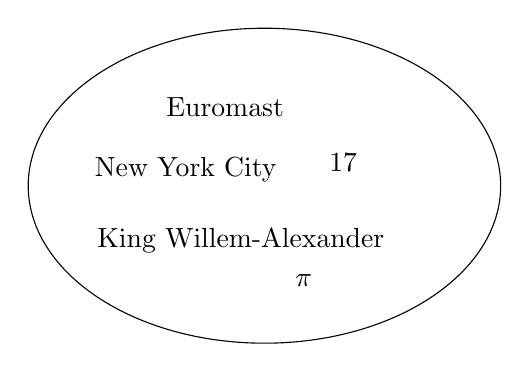
\begin{tikzpicture}
\draw (0,0) ellipse (3cm and 2cm);
\node at (-0.5, 1.0) {Euromast};
\node at (-1.0, 0.2) {New York City};
\node at (1.0, 0.3) {17};
\node at (-0.3, -0.7) {King Willem-Alexander};
\node at (0.5, -1.2) {$\pi$};
\end{tikzpicture}
\caption{Biểu đồ Venn của một tập hợp ví dụ.}
\label{fig:4.1}
\end{figure}

Phép toán cơ bản nhất trong lý thuyết tập hợp là tạo một tập hợp từ một danh sách cho trước các thực thể cụ thể. Tập hợp được tạo theo cách này được ký hiệu bằng cách bao danh sách các thực thể giữa một dấu ngoặc nhọn trái, `$\{$', và một dấu ngoặc nhọn phải, `$\}$'. Các thực thể trong danh sách được phân cách bởi dấu phẩy. Ví dụ, tập hợp được ký hiệu bởi
\[
\{ 17,\; \pi,\; \text{New York City},\; \text{King Willem-Alexander},\; \text{Euromast} \}
\]
là tập hợp chứa các thực thể $17$, $\pi$, New York City, King Willem-Alexander, và Euromast. Các thực thể này là các \textbf{phần tử} của tập hợp. Hình~\ref{fig:4.1} là một mô tả trừu tượng của tập hợp này.

Vì chúng ta giả định rằng một tập hợp được xác định hoàn toàn bởi các phần tử mà nó chứa, nên tập hợp là xác định. Tất nhiên, chúng ta vẫn chưa nói ``thực thể'' nghĩa là gì. Một thứ gì đó xác định như ``New York City'' có thể đủ tư cách, ngoại trừ việc dường như New York City không thực sự thuộc về thế giới toán học. Vấn đề là toán học được cho là thế giới khép kín của riêng nó, nhưng nó lại phải mô hình hóa thế giới thực. Khi chúng ta sử dụng toán học để mô hình hóa thế giới thực, chúng ta chấp nhận các thực thể như New York City và thậm chí Euromast. Nhưng khi chúng ta làm toán thuần túy, chúng ta thường chỉ dùng các thực thể toán học rõ ràng như số nguyên $17$ hay số thực $\pi$. Chúng ta cũng sẽ sử dụng các chữ cái như $a$ và $b$ để chỉ các thực thể. Ví dụ, khi chúng ta nói ``Cho $A$ là tập hợp $\{a, b, c\}$'', chúng ta muốn nói $a$, $b$, và $c$ là các thực thể cụ thể nhưng không được chỉ rõ.

\begin{warningbox}
Điều quan trọng cần hiểu là một tập hợp được xác định bởi các phần tử mà nó chứa, chứ không phải bởi thứ tự mà các phần tử được liệt kê. Ví dụ, các ký hiệu $\{a, b, c, d\}$ và $\{b, c, a, d\}$ định nghĩa cùng một tập hợp. Hơn nữa, một tập hợp chỉ có thể chứa một bản sao của một phần tử cho trước, ngay cả khi ký hiệu đặc tả tập hợp liệt kê phần tử đó hai lần. Điều này có nghĩa là $\{a, b, a, a, b, c, a\}$ và $\{a, b, c\}$ chỉ cùng một tập hợp. Lưu ý đặc biệt rằng nói tập hợp $\{a, b, a, a, b, c, a\}$ chứa bảy phần tử là không chính xác, vì một số phần tử trong danh sách là giống hệt nhau. Ký hiệu $\{a, b, c\}$ có thể gây nhầm lẫn, vì có thể không rõ liệu các chữ cái $a$, $b$, và $c$ có được giả định là chỉ ba thực thể khác nhau hay không. Một nhà toán học thường sẽ không đưa ra giả định này mà không phát biểu nó một cách rõ ràng, sao cho tập hợp được ký hiệu bởi $\{a, b, c\}$ thực tế có thể chứa một, hai, hoặc ba phần tử. Khi điều quan trọng là các chữ cái khác nhau chỉ các thực thể khác nhau, chúng ta sẽ nói rõ ràng, như trong ``Xét tập hợp $\{a, b, c\}$, trong đó $a$, $b$, và $c$ là phân biệt.''
\end{warningbox}

\subsection{Phần tử của tập hợp}

Ký hiệu $\in$ được dùng để biểu thị quan hệ ``là một phần tử của''. Nghĩa là, nếu $a$ là một thực thể và $A$ là một tập hợp, thì $a \in A$ là một mệnh đề đúng khi và chỉ khi $a$ là một trong các phần tử của $A$. Trong trường hợp đó, chúng ta cũng nói rằng $a$ là một \textbf{thành viên} của tập hợp $A$. Khẳng định rằng $a$ không phải là phần tử của $A$ được biểu thị bằng ký hiệu $a \notin A$. Lưu ý rằng cả $a \in A$ và $a \notin A$ đều là các mệnh đề theo nghĩa của logic mệnh đề. Nghĩa là, chúng là các khẳng định có thể đúng hoặc sai. Mệnh đề $a \notin A$ tương đương với $\neg(a \in A)$.

\begin{notebox}
Như bạn có thể đã nhận thấy, quy ước là tập hợp được ký hiệu bằng chữ cái viết hoa (ví dụ `$A$') và các phần tử trong tập hợp được ký hiệu bằng chữ cái viết thường (ví dụ `$a$'). Bạn nên tuân theo quy ước tương tự để tránh hiểu lầm!
\end{notebox}

Một tập hợp có thể rỗng, nghĩa là không chứa phần tử nào cả. Vì một tập hợp được xác định hoàn toàn bởi các phần tử mà nó chứa, nên chỉ có một tập hợp không chứa phần tử nào. Tập hợp này được gọi là \textbf{tập rỗng}, và nó được ký hiệu bằng ký hiệu $\varnothing$. Lưu ý rằng với mọi phần tử $a$, mệnh đề $a \in \varnothing$ là sai. Tập rỗng $\varnothing$ cũng có thể được ký hiệu bằng một cặp ngoặc nhọn rỗng, tức là $\{\}$.

Nếu $A$ và $B$ là các tập hợp, thì theo định nghĩa, $A$ \textbf{bằng} $B$ khi và chỉ khi chúng chứa chính xác cùng các phần tử. Trong trường hợp này, chúng ta viết $A = B$. Sử dụng ký hiệu của logic vị từ, chúng ta có thể nói rằng $A = B$ khi và chỉ khi $\forall x\,(x \in A \leftrightarrow x \in B)$.

\begin{warningbox}
Sau này, khi chứng minh các định lý trong lý thuyết tập hợp, chúng ta sẽ thấy rằng việc sử dụng ký hiệu logic vị từ này thường giúp đơn giản hóa các chứng minh. Để tránh phải tra cứu lại sau này, hãy chắc chắn rằng bạn hiểu tại sao ký hiệu logic vị từ tương đương với ký hiệu tập hợp.
\end{warningbox}

Bây giờ giả sử rằng $A$ và $B$ là các tập hợp sao cho mọi phần tử của $A$ đều là phần tử của $B$. Trong trường hợp đó, chúng ta nói rằng $A$ là \textbf{tập con} của $B$, tức là $A$ là tập con của $B$ khi và chỉ khi $\forall x\,(x \in A \to x \in B)$. Sự kiện $A$ là tập con của $B$ được ký hiệu bởi $A \subseteq B$. Lưu ý rằng $\varnothing$ là tập con của mọi tập hợp $B$: $x \in \varnothing$ là sai với mọi $x$, và do đó với mọi $B$, $(x \in \varnothing \to x \in B)$ là đúng với mọi $x$.

Nếu $A = B$, thì tự động đúng rằng $A \subseteq B$ và $B \subseteq A$. Mệnh đề đảo cũng đúng: Nếu $A \subseteq B$ và $B \subseteq A$, thì $A = B$. Điều này suy ra từ sự kiện rằng với mọi $x$, mệnh đề $(x \in A \leftrightarrow x \in B)$ tương đương logic với mệnh đề $(x \in A \to x \in B) \land (x \in B \to x \in A)$. Sự kiện này đủ quan trọng để phát biểu thành một định lý.

\begin{theorem}
\label{thm:4.1}
Cho $A$ và $B$ là các tập hợp. Khi đó $A = B$ khi và chỉ khi $A \subseteq B$ và $B \subseteq A$.
\end{theorem}

Định lý này biểu đạt lời khuyên sau: Nếu bạn muốn kiểm tra rằng hai tập hợp $A$ và $B$ bằng nhau, bạn có thể làm điều đó trong hai bước. Đầu tiên kiểm tra rằng mọi phần tử của $A$ cũng là phần tử của $B$, và sau đó kiểm tra rằng mọi phần tử của $B$ cũng là phần tử của $A$.

Nếu $A \subseteq B$ nhưng $A \neq B$, chúng ta nói rằng $A$ là \textbf{tập con thực sự} của $B$. Chúng ta dùng ký hiệu $A \subsetneq B$ để chỉ rằng $A$ là tập con thực sự của $B$. Nghĩa là, $A \subsetneq B$ khi và chỉ khi $A \subseteq B \land A \neq B$. Đôi khi chúng ta sẽ dùng $A \supseteq B$ như một ký hiệu tương đương cho $B \subseteq A$, và $A \supsetneq B$ như tương đương cho $B \subsetneq A$. Các sách giáo khoa khác đôi khi cũng dùng ký hiệu $\subset$ để biểu thị tập con thực sự, ví dụ $A \subset B \equiv A \subsetneq B$. Ngoài ra, bạn có thể gặp $A \not\subseteq B$ có nghĩa là $A$ không phải là tập con của $B$. Lưu ý rằng (đặc biệt trong văn bản viết tay) sự khác biệt giữa $A \subsetneq B$ và $A \not\subseteq B$ có thể rất nhỏ, vì vậy hãy đọc cẩn thận và viết rõ ràng!

\subsection{Ký hiệu xây dựng tập hợp}

Một tập hợp có thể chứa vô hạn phần tử. Trong trường hợp đó, không thể liệt kê tất cả các phần tử trong tập hợp: chúng ta không thể đưa ra một \textit{định nghĩa ngoại diên} của tập hợp. Đôi khi dấu ba chấm `$\ldots$' được dùng để chỉ một danh sách tiếp tục vô hạn. Ví dụ, $\mathbb{N}$, tập hợp các số tự nhiên, có thể được đặc tả là
\[
\mathbb{N} = \{0, 1, 2, 3, \ldots\}
\]
Tuy nhiên, đây là một ký hiệu không chính thức, không thực sự được xác định chặt chẽ, và chỉ nên dùng trong trường hợp ý nghĩa của nó rõ ràng. Không hữu ích lắm khi nói rằng ``tập hợp các số nguyên tố là $\{2, 3, 5, 7, 11, 13, \ldots\}$'', và hoàn toàn vô nghĩa khi nói về ``tập hợp $\{17, 42, 105, \ldots\}$''. Rõ ràng, chúng ta cần một cách khác để đặc tả tập hợp ngoài việc liệt kê các phần tử. Nhu cầu này được đáp ứng bởi các vị từ.

Nếu $P(x)$ là một vị từ, thì chúng ta có thể tạo tập hợp chứa tất cả các thực thể $a$ sao cho $a$ nằm trong miền diễn giải của $P$ và $P(a)$ là đúng. Ký hiệu $\{x \mid P(x)\}$ được dùng để chỉ tập hợp này. Đây là \textit{định nghĩa nội hàm} của tập hợp. Tên của biến, $x$, là tùy ý, nên cùng một tập hợp có thể được ký hiệu tương đương là $\{z \mid P(z)\}$ hoặc $\{r \mid P(r)\}$. Ký hiệu $\{x \mid P(x)\}$ có thể được đọc là ``tập hợp các $x$ sao cho $P(x)$''. Chúng ta gọi đây là \textbf{ký hiệu xây dựng tập hợp}, vì bạn có thể nghĩ về vị từ như một vật liệu xây dựng cho các phần tử của tập hợp. Ví dụ, nếu $E(x)$ là vị từ `$x$ là số chẵn', và nếu miền diễn giải của $E$ là tập $\mathbb{N}$, thì ký hiệu $\{x \mid E(x)\}$ đặc tả tập hợp các số tự nhiên chẵn. Nghĩa là,
\[
\{x \mid E(x)\} = \{0, 2, 4, 6, 8, \ldots\}
\]

\begin{infobox}
Hóa ra, vì những lý do sâu xa và đáng ngạc nhiên mà chúng ta sẽ thảo luận sau, chúng ta phải cẩn thận một chút về những gì được coi là một vị từ. Để ký hiệu $\{x \mid P(x)\}$ có nghĩa, chúng ta phải giả định rằng miền diễn giải của $P$ thực sự là một tập hợp. (Bạn có thể thắc mắc làm sao nó có thể là thứ khác. Đó chính là điều đáng ngạc nhiên!)
\end{infobox}

Thường thì việc chỉ rõ miền diễn giải trong ký hiệu định nghĩa tập hợp là hữu ích. Trong ví dụ trên, để làm rõ rằng $x$ phải là số tự nhiên, chúng ta có thể viết tập hợp dưới dạng $\{x \in \mathbb{N} \mid E(x)\}$. Ký hiệu này có thể được đọc là ``tập hợp tất cả $x$ trong $\mathbb{N}$ sao cho $E(x)$''. Tổng quát hơn, nếu $X$ là một tập hợp và $P$ là một vị từ có miền diễn giải bao gồm tất cả các phần tử của $X$, thì ký hiệu
\[
\{x \in X \mid P(x)\}
\]
là tập hợp gồm tất cả các thực thể $a$ là thành viên của tập $X$ và thỏa mãn $P(a)$ là đúng. Trong ký hiệu này, chúng ta không cần giả định rằng miền diễn giải của $P$ là một tập hợp, vì chúng ta đang hạn chế miền diễn giải vào tập $X$. Tập hợp được ký hiệu bởi $\{x \in X \mid P(x)\}$ cũng có thể được viết là $\{x \mid x \in X \land P(x)\}$.

\begin{example}
Chúng ta có thể sử dụng ký hiệu này để định nghĩa tập hợp các số nguyên tố một cách chặt chẽ. Một số nguyên tố là một số tự nhiên $n$ lớn hơn $1$ và thỏa mãn tính chất rằng với mọi phân tích $n = xy$, trong đó $x$ và $y$ là các số tự nhiên, thì $x$ hoặc $y$ phải bằng $n$. Chúng ta có thể biểu diễn định nghĩa này dưới dạng vị từ và định nghĩa tập hợp các số nguyên tố là
\[
\{n \in \mathbb{N} \mid (n > 1) \land \forall x\,\forall y\,\bigl((x \in \mathbb{N} \land y \in \mathbb{N} \land n = xy) \to (x = n \lor y = n)\bigr)\}
\]
Phải thừa nhận rằng định nghĩa này khó nuốt trôi trong một lần. Nhưng ví dụ này cho thấy rằng có thể định nghĩa các tập hợp phức tạp bằng vị từ.
\end{example}

\subsection{Các phép toán trên tập hợp}

Bây giờ chúng ta đã có cách biểu diễn nhiều loại tập hợp khác nhau, chúng ta chuyển sang các phép toán có thể thực hiện trên tập hợp. Các phép toán cơ bản nhất trên tập hợp là \textbf{hợp} và \textbf{giao}. Nếu $A$ và $B$ là các tập hợp, thì chúng ta định nghĩa \textbf{hợp} của $A$ và $B$ là tập hợp chứa tất cả các phần tử của $A$ cùng với tất cả các phần tử của $B$. Hợp của $A$ và $B$ được ký hiệu bởi $A \cup B$. Hợp có thể được định nghĩa chính thức là
\[
A \cup B = \{x \mid x \in A \lor x \in B\}.
\]
\textbf{Giao} của $A$ và $B$ được định nghĩa là tập hợp chứa mọi thực thể vừa là thành viên của $A$ vừa là thành viên của $B$. Giao của $A$ và $B$ được ký hiệu bởi $A \cap B$. Chính thức,
\[
A \cap B = \{x \mid x \in A \land x \in B\}.
\]
Một thực thể thuộc $A \cup B$ nếu nó nằm trong $A$ \textit{hoặc} $B$. Nó thuộc $A \cap B$ nếu nó nằm trong \textit{cả} $A$ \textit{và} $B$. Lưu ý rằng ký hiệu cho toán tử logic ``hoặc'', $\lor$, tương tự với ký hiệu cho toán tử hợp, $\cup$, trong khi toán tử logic ``và'', $\land$, tương tự với toán tử giao, $\cap$.

\textbf{Hiệu tập hợp} của hai tập hợp $A$ và $B$ được định nghĩa là tập hợp tất cả các thực thể là thành viên của $A$ nhưng không phải thành viên của $B$. Hiệu tập hợp của $A$ và $B$ được ký hiệu $A \setminus B$ hoặc $A - B$. Ý tưởng là $A \setminus B$ được tạo bằng cách bắt đầu với $A$ và sau đó loại bỏ bất kỳ phần tử nào cũng có mặt trong $B$. Chính thức,
\[
A \setminus B = \{x \mid x \in A \land x \notin B\}.
\]

Hợp và giao rõ ràng là các phép toán giao hoán. Nghĩa là, $A \cup B = B \cup A$ và $A \cap B = B \cap A$ với mọi tập hợp $A$ và $B$. Tuy nhiên, hiệu tập hợp không giao hoán. Nói chung, $A \setminus B \neq B \setminus A$.

\begin{example}
Giả sử rằng $A = \{a, b, c\}$, $B = \{b, d\}$, và $C = \{d, e, f\}$. Khi đó chúng ta có thể áp dụng các định nghĩa của hợp, giao, và hiệu tập hợp để tính, ví dụ:
\begin{align*}
A \cup B &= \{a, b, c, d\}  &  A \cap B &= \{b\}  &  A \setminus B &= \{a, c\} \\
A \cup C &= \{a, b, c, d, e, f\}  &  A \cap C &= \varnothing  &  A \setminus C &= \{a, b, c\}
\end{align*}
\end{example}

Trong ví dụ này, các tập hợp $A$ và $C$ không có phần tử chung, nên $A \cap C = \varnothing$. Có một thuật ngữ cho điều này: Hai tập hợp được gọi là \textbf{rời nhau} nếu chúng không có phần tử chung. Nghĩa là, với mọi tập hợp $A$ và $B$, $A$ và $B$ được gọi là rời nhau khi và chỉ khi $A \cap B = \varnothing$.

Tất nhiên, các phép toán tập hợp cũng có thể được áp dụng cho các tập hợp được định nghĩa bằng vị từ. Ví dụ tiếp theo minh họa điều này.

\begin{example}
Cho $L(x)$ là vị từ `$x$ may mắn', và cho $W(x)$ là vị từ `$x$ khôn ngoan', trong đó miền diễn giải của mỗi vị từ là tập hợp người. Cho $X = \{x \mid L(x)\}$, và cho $Y = \{x \mid W(x)\}$. Khi đó
\begin{align*}
X \cup Y &= \{x \mid L(x) \lor W(x)\} = \{\text{người may mắn hoặc khôn ngoan}\} \\
X \cap Y &= \{x \mid L(x) \land W(x)\} = \{\text{người may mắn và khôn ngoan}\} \\
X \setminus Y &= \{x \mid L(x) \land \neg W(x)\} = \{\text{người may mắn nhưng không khôn ngoan}\} \\
Y \setminus X &= \{x \mid W(x) \land \neg L(x)\} = \{\text{người khôn ngoan nhưng không may mắn}\}
\end{align*}
\end{example}

\begin{warningbox}
Bạn phải cẩn thận một chút với từ ``và'' trong tiếng Việt (hay ``and'' trong tiếng Anh). Chúng ta có thể nói rằng tập $X \cup Y$ chứa những người may mắn \textit{và} những người khôn ngoan. Nhưng điều đó có nghĩa là một người thuộc tập $X \cup Y$ bằng cách may mắn \textit{hoặc} bằng cách khôn ngoan, nên $X \cup Y$ được định nghĩa bằng toán tử logic ``hoặc'', $\lor$.
\end{warningbox}

\subsection{Trực quan hóa tập hợp\protect\footnote{Tiểu mục này được suy ra từ en.wikipedia.org/wiki/Venn\_diagram.}}

Việc trực quan hóa tập hợp có thể rất hữu ích. \textbf{Biểu đồ Venn} thể hiện tất cả các quan hệ logic có thể có giữa một tập hợp hữu hạn các tập hợp khác nhau. Các biểu đồ này mô tả các phần tử như các điểm trong mặt phẳng, và các tập hợp như các miền bên trong các đường cong khép kín. Vì vậy một biểu đồ Venn gồm nhiều đường cong khép kín chồng lên nhau, thường là các hình tròn, mỗi hình biểu diễn một tập hợp. Các điểm bên trong đường cong (hình tròn) được gán nhãn $S$ biểu diễn các phần tử của tập hợp $S$, trong khi các điểm bên ngoài biên biểu diễn các phần tử không thuộc tập $S$. Hình~\ref{fig:4.1} thể hiện tập hợp ví dụ mở đầu phần này.

% Hình 4.3: Biểu đồ Venn của giao hai tập hợp
\begin{figure}[ht]
\centering
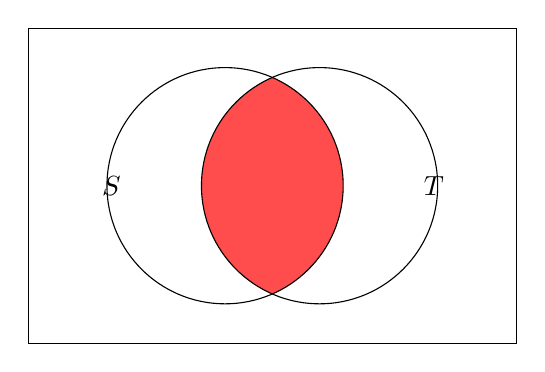
\begin{tikzpicture}
\begin{scope}
\clip (0,0) circle (1.5cm);
\fill[red!70] (1.2,0) circle (1.5cm);
\end{scope}
\draw (0,0) circle (1.5cm) node[left=1.2cm] {$S$};
\draw (1.2,0) circle (1.5cm) node[right=1.2cm] {$T$};
\draw (-2.5,-2) rectangle (3.7,2);
\end{tikzpicture}
\caption{Biểu đồ Venn của giao hai tập hợp.}
\label{fig:4.3}
\end{figure}

Biểu đồ Venn giúp chúng ta trực quan hóa các tập hợp và các phép toán tập hợp. Ví dụ, tập hợp tất cả các phần tử thuộc cả hai tập $S$ và $T$, $S \cap T$, được biểu diễn trực quan bởi vùng giao nhau của các miền $S$ và $T$: xem Hình~\ref{fig:4.3}. Trong biểu đồ Venn, các đường cong được chồng lên nhau theo mọi cách có thể, thể hiện tất cả các quan hệ có thể giữa các tập hợp. Bạn có thể thấy hữu ích khi vẽ biểu đồ Venn để có trực giác về những gì đang xảy ra. Tuy nhiên, biểu đồ Venn tự nó không cung cấp chứng minh cho các định lý trong lý thuyết tập hợp.

% Bảng ký hiệu - Hình 4.2
\begin{figure}[ht]
\centering
\begin{tabular}{cl}
\toprule
\textbf{Ký hiệu} & \textbf{Định nghĩa} \\
\midrule
$a \in A$ & $a$ là thành viên (hay phần tử) của $A$ \\
$a \notin A$ & $\neg(a \in A)$, $a$ không phải thành viên của $A$ \\
$\varnothing$ & tập rỗng, không chứa phần tử nào \\
$A \subseteq B$ & $A$ là tập con của $B$, $\forall x\,(x \in A \to x \in B)$ \\
$A \subsetneq B$ & $A$ là tập con thực sự của $B$, $A \subseteq B \land A \neq B$ \\
$A \supseteq B$ & $A$ là tập chứa của $B$, tương đương $B \subseteq A$ \\
$A \supsetneq B$ & $A$ là tập chứa thực sự của $B$, tương đương $B \subsetneq A$ \\
$A = B$ & $A$ và $B$ có cùng các thành viên, $A \subseteq B \land B \subseteq A$ \\
$A \cup B$ & hợp của $A$ và $B$, $\{x \mid x \in A \lor x \in B\}$ \\
$A \cap B$ & giao của $A$ và $B$, $\{x \mid x \in A \land x \in B\}$ \\
$A \setminus B$ & hiệu tập hợp của $A$ và $B$, $\{x \mid x \in A \land x \notin B\}$ \\
$A \triangle B$ & hiệu đối xứng của $A$ và $B$, $\{x \mid (x \in A \land x \notin B) \lor (x \notin A \land x \in B)\}$ \\
$\mathcal{P}(A)$ & tập lũy thừa của $A$, $\{X \mid X \subseteq A\}$ \\
\bottomrule
\end{tabular}
\caption{Một số ký hiệu được định nghĩa trong mục này. $A$ và $B$ là các tập hợp, và $a$ là một thực thể.}
\label{fig:4.2}
\end{figure}

\subsection{Tập hợp của tập hợp}

Tập hợp có thể chứa các tập hợp khác làm phần tử. Ví dụ, ký hiệu $\{a, \{b\}\}$ định nghĩa một tập hợp chứa hai phần tử, thực thể $a$ và tập hợp $\{b\}$. Vì tập $\{b\}$ là thành viên của tập $\{a, \{b\}\}$, chúng ta có $\{b\} \in \{a, \{b\}\}$. Mặt khác, nếu $a \neq b$, mệnh đề $\{b\} \subseteq \{a, \{b\}\}$ là sai, vì nói $\{b\} \subseteq \{a, \{b\}\}$ tương đương với nói rằng $b \in \{a, \{b\}\}$, và thực thể $b$ không phải là một trong hai thành viên của $\{a, \{b\}\}$. Với thực thể $a$, đúng rằng $\{a\} \subseteq \{a, \{b\}\}$ và với tập $\{b\}$, đúng rằng $\{\{b\}\} \subseteq \{a, \{b\}\}$. Hãy nghiên cứu các ví dụ này cẩn thận trước khi tiếp tục, vì nhiều sinh viên gặp khó khăn với khái niệm và ký hiệu của việc đặt tập hợp trong tập hợp.

Cho một tập hợp $A$, chúng ta có thể xây dựng tập hợp chứa tất cả các tập con của $A$. Tập hợp này được gọi là \textbf{tập lũy thừa} của $A$, và được ký hiệu $\mathcal{P}(A)$. Chính thức, chúng ta định nghĩa
\[
\mathcal{P}(A) = \{X \mid X \subseteq A\}.
\]

\begin{example}
Ví dụ, nếu $A = \{a, b\}$, thì các tập con của $A$ là tập rỗng, $\{a\}$, $\{b\}$, và $\{a, b\}$, nên tập lũy thừa của $A$ là tập cho bởi
\[
\mathcal{P}(A) = \{\varnothing, \{a\}, \{b\}, \{a, b\}\}.
\]
Vậy tập lũy thừa của $A$ có bốn phần tử. Điều này có làm bạn ngạc nhiên không?
\end{example}

Lưu ý rằng vì tập rỗng là tập con của mọi tập hợp, tập rỗng là một phần tử của tập lũy thừa của mọi tập hợp. Nghĩa là, với mọi tập $A$, $\varnothing \subseteq A$ và $\varnothing \in \mathcal{P}(A)$. Vì tập rỗng là tập con của chính nó, và là tập con duy nhất của nó, chúng ta có $\mathcal{P}(\varnothing) = \{\varnothing\}$. Tập $\{\varnothing\}$ không rỗng. Nó chứa một phần tử, cụ thể là $\varnothing$.

\begin{infobox}
Giải Nobel đã được trao cho Bertrand Russell (1872--1970), một nhân vật thống trị trong tư tưởng Anh quốc trong thế kỷ hai mươi. Russell là một triết gia và nhà toán học, đồng thời cũng là nhà sử học, nhà phê bình xã hội và nhà hoạt động chính trị. Cùng với A.\,N. Whitehead, Russell đã viết \textit{Principia Mathematica}, một nỗ lực hoành tráng nhằm tạo ra cơ sở logic cho toán học. Công trình của ông đã có ảnh hưởng đáng kể đến khoa học máy tính, không chỉ vì những đóng góp cho logic và lý thuyết tập hợp: ông đã đề xuất những manh nha của cái ngày nay gọi là \textit{hệ thống kiểu}.

\noindent Nguồn: en.wikipedia.org/wiki/Bertrand\_Russell.
\end{infobox}

Chúng ta đã nhận xét trước đó trong mục này rằng ký hiệu $\{x \mid P(x)\}$ chỉ hợp lệ khi miền diễn giải của $P$ là một tập hợp. Điều này có vẻ khá khó hiểu --- xét cho cùng, tại sao và làm thế nào miền diễn giải lại có thể là thứ khác? Câu trả lời liên quan đến \textbf{Nghịch lý Russell}, mà chúng ta đã nhắc đến ngắn gọn ở Chương~3 và cho thấy rằng tập hợp của tất cả các tập hợp không thể tồn tại về mặt logic. Tính bất khả thi này có thể được chứng minh bằng phản chứng. Trong chứng minh, chúng ta sử dụng sự tồn tại của tập hợp mọi tập hợp để định nghĩa một tập hợp khác không thể tồn tại vì sự tồn tại của nó sẽ dẫn đến mâu thuẫn logic.

\begin{theorem}
\label{thm:4.2}
Không tồn tại tập hợp của tất cả các tập hợp.
\end{theorem}

\begin{proof}
Giả sử rằng tập hợp của tất cả các tập hợp tồn tại. Chúng ta sẽ chỉ ra rằng giả thiết này dẫn đến mâu thuẫn. Gọi $V$ là tập hợp của tất cả các tập hợp. Khi đó chúng ta có thể định nghĩa tập $R$ là tập chứa mọi tập hợp mà không chứa chính nó. Nghĩa là,
\[
R = \{X \in V \mid X \notin X\}
\]
Bây giờ, chúng ta phải có hoặc $R \in R$ hoặc $R \notin R$. Chúng ta sẽ chỉ ra rằng cả hai trường hợp đều dẫn đến mâu thuẫn.

Xét trường hợp $R \in R$. Vì $R \in R$, $R$ phải thỏa mãn điều kiện thành viên trong $R$. Một tập $X$ thuộc $R$ khi và chỉ khi $X \notin X$. Nói rằng $R$ thỏa mãn điều kiện này có nghĩa là $R \notin R$. Nghĩa là, từ sự kiện $R \in R$, chúng ta suy ra mâu thuẫn $R \notin R$.

Bây giờ xét trường hợp còn lại, $R \notin R$. Vì $R \notin R$, $R$ không thỏa mãn điều kiện thành viên trong $R$. Vì điều kiện thành viên là $R \notin R$, và điều kiện này là sai, mệnh đề $R \notin R$ phải là sai. Nhưng điều này có nghĩa là mệnh đề $R \in R$ là đúng. Từ sự kiện $R \notin R$, chúng ta suy ra mâu thuẫn $R \in R$.

Vì cả hai trường hợp có thể, $R \in R$ và $R \notin R$, đều dẫn đến mâu thuẫn, chúng ta thấy rằng $R$ không thể tồn tại. Vì sự tồn tại của $R$ suy ra từ sự tồn tại của $V$, chúng ta thấy rằng $V$ cũng không thể tồn tại.
\end{proof}

\begin{notebox}
Mâu thuẫn (khét tiếng) này đã được chuyển thể sang ngôn ngữ tự nhiên để giúp người không chuyên dễ hiểu hơn. Thật không may, nhiều bản dịch như vậy có sai sót. Bạn có thể nghĩ ra lời giải cho câu sau không? ``Thợ cắt tóc của Seville cắt tóc cho tất cả đàn ông không tự cắt tóc. Ai cắt tóc cho thợ cắt tóc?''
\end{notebox}

Để tránh Nghịch lý Russell, chúng ta phải đặt các giới hạn lên việc xây dựng các tập hợp mới. Chúng ta không thể ép tập hợp mọi tập hợp tồn tại chỉ bằng cách nghĩ về nó. Chúng ta không thể tạo tập hợp $\{x \mid P(x)\}$ trừ khi miền diễn giải của $P$ là một tập hợp. Bất kỳ vị từ $Q$ nào cũng có thể được dùng để tạo tập hợp $\{x \in X \mid Q(x)\}$, nhưng ký hiệu này đòi hỏi một tập hợp $X$ đã tồn tại từ trước. Các vị từ có thể được dùng để tạo tập con của các tập hợp đã tồn tại, nhưng chúng không thể được dùng để tạo tập hợp mới hoàn toàn từ đầu.

Ký hiệu $\{x \in A \mid P(x)\}$ là cách thuận tiện để hạn chế miền diễn giải của vị từ $P$ vào các thành viên của tập $A$ mà chúng ta thực sự quan tâm. Chúng ta sẽ dùng ký hiệu tương tự với các lượng từ $\forall$ và $\exists$. Mệnh đề $(\forall x \in A)(P(x))$ đúng khi và chỉ khi $P(a)$ đúng với mọi phần tử $a$ của tập $A$. Và mệnh đề $(\exists x \in A)(P(x))$ đúng khi và chỉ khi tồn tại phần tử $a$ nào đó của tập $A$ sao cho $P(a)$ đúng. Các ký hiệu này chỉ hợp lệ khi $A$ nằm trong miền diễn giải của $P$. Như thường lệ, chúng ta có thể bỏ ngoặc khi làm vậy không gây nhập nhằng. Vậy ví dụ chúng ta có thể viết $\forall x \in A\; P(x)$.

\subsection{Bộ sưu tập có thứ tự: Bộ}

Nếu $a$ và $b$ là các thực thể, thì $(a, b)$ ký hiệu \textbf{cặp có thứ tự} chứa $a$ và $b$. Cặp có thứ tự $(a, b)$ khác với tập hợp $\{a, b\}$ vì tập hợp không có thứ tự. Nghĩa là, $\{a, b\}$ và $\{b, a\}$ ký hiệu cùng một tập hợp, nhưng nếu $a \neq b$, thì $(a, b)$ và $(b, a)$ là các cặp có thứ tự khác nhau. Tổng quát hơn, hai cặp có thứ tự $(a, b)$ và $(c, d)$ bằng nhau khi và chỉ khi $a = c$ và $b = d$. Nếu $(a, b)$ là một cặp có thứ tự, thì $a$ và $b$ được gọi là các \textbf{tọa độ} của cặp có thứ tự. Cụ thể, $a$ là tọa độ thứ nhất và $b$ là tọa độ thứ hai.

\begin{notebox}
Ở trung học, bạn cũng phải viết tọa độ $(x,y)$ sử dụng ký hiệu cặp có thứ tự này. Ví dụ bạn sẽ nói rằng đường thẳng $y = ax + b$ cắt trục $y$ tại $(0, b)$ và trục $x$ tại $(-\frac{b}{a}, 0)$.
\end{notebox}

Bạn có thể mở rộng khái niệm này cho nhiều hơn chỉ các cặp. Với ba phần tử chúng ta có thể tạo \textbf{bộ ba có thứ tự} $(a, b, c)$. Định nghĩa cho bốn hoặc nhiều tọa độ hơn là tương tự. Thuật ngữ chung cho một bộ sưu tập có thứ tự như vậy là \textbf{bộ} (tuple) hay chính xác hơn, \textbf{bộ $n$ có thứ tự}. Ví dụ, $(a, b, c, d, e)$ là một bộ 5 có thứ tự.

\subsection{Thêm một phép toán tập hợp: Tích Descartes}

Nếu $A$ và $B$ là các tập hợp, thì chúng ta có thể tạo tập $A \times B$ được định nghĩa bởi
\[
A \times B = \{(a, b) \mid a \in A \text{ và } b \in B\}.
\]
Tập hợp này được gọi là \textbf{tích chéo} hay \textbf{tích Descartes} của các tập $A$ và $B$. Tập $A \times B$ chứa mọi cặp có thứ tự mà tọa độ thứ nhất là phần tử của $A$ và tọa độ thứ hai là phần tử của $B$. Ví dụ, nếu $X = \{c, d\}$ và $Y = \{1, 2, 3\}$, thì $X \times Y = \{(c,1), (c,2), (c,3), (d,1), (d,2), (d,3)\}$.

Có thể mở rộng ý tưởng này cho tích Descartes của nhiều hơn hai tập hợp. Tích Descartes của ba tập $A$, $B$, và $C$ được ký hiệu $A \times B \times C$ và tạo ra các bộ ba có thứ tự $(a, b, c)$ trong đó $a \in A$, $b \in B$, $c \in C$. Một ví dụ khác có thể tìm thấy trong các cặp bạn cùng làm bài tập mà bạn đã tạo cho môn học này. Mỗi cặp sinh viên này là một bộ 2, từ tập $S \times S$ trong đó $S$ là tập hợp các sinh viên đang học môn \textit{Lập luận \& Logic}.

\subsection{Quy nạp toán học -- xem lại}

Chúng ta kết thúc mục này bằng cách quay lại chủ đề quy nạp toán học. Đầu tiên, chúng ta sẽ đưa ra các chứng minh cho hai dạng của nguyên lý quy nạp toán học. Các chứng minh này đã bị bỏ qua ở chương trước, nhưng chỉ vì thiếu một chút ký hiệu tập hợp. Trên thực tế, nguyên lý quy nạp toán học chỉ có hiệu lực vì nó suy ra từ một trong những tiên đề cơ bản định nghĩa các số tự nhiên, cụ thể là sự kiện rằng mọi tập con không rỗng của các số tự nhiên đều có phần tử nhỏ nhất. Với tiên đề này, chúng ta có thể dùng nó để chứng minh hai định lý sau:

\begin{theorem}
\label{thm:4.3}
Cho $P$ là vị từ một ngôi có miền diễn giải bao gồm các số tự nhiên. Giả sử rằng $P(0) \land \bigl(\forall k \in \mathbb{N}\;(P(k) \to P(k+1))\bigr)$. Khi đó $\forall n \in \mathbb{N},\; P(n)$.
\end{theorem}

\begin{proof}
Giả sử rằng cả $P(0)$ và $\forall k \in \mathbb{N}\;(P(k) \to P(k+1))$ đều đúng, nhưng $\forall n \in \mathbb{N},\; P(n)$ là sai. Chúng ta chỉ ra rằng giả thiết này dẫn đến mâu thuẫn.

Vì mệnh đề $\forall n \in \mathbb{N},\; P(n)$ là sai, phủ định của nó, $\neg(\forall n \in \mathbb{N},\; P(n))$, là đúng. Phủ định này tương đương với $\exists n \in \mathbb{N},\; \neg P(n)$. Đặt $X = \{n \in \mathbb{N} \mid \neg P(n)\}$. Vì $\exists n \in \mathbb{N},\; \neg P(n)$ đúng, chúng ta biết rằng $X$ không rỗng. Vì $X$ là tập con không rỗng của các số tự nhiên, nó có phần tử nhỏ nhất. Gọi $x$ là phần tử nhỏ nhất của $X$. Nghĩa là, $x$ là số tự nhiên nhỏ nhất sao cho $P(x)$ sai. Vì chúng ta biết $P(0)$ đúng, $x$ không thể là $0$. Đặt $y = x - 1$. Vì $x \neq 0$, $y$ là một số tự nhiên. Vì $y < x$, theo định nghĩa của $x$, chúng ta biết rằng $P(y)$ đúng. Chúng ta cũng biết rằng $\forall k \in \mathbb{N}\;(P(k) \to P(k+1))$ đúng. Cụ thể, lấy $k = y$, chúng ta biết rằng $P(y) \to P(y+1)$. Vì $P(y)$ và $P(y) \to P(y+1)$, theo modus ponens chúng ta suy ra $P(y+1)$ đúng. Nhưng $y + 1 = x$, nên chúng ta đã suy ra rằng $P(x)$ đúng. Điều này mâu thuẫn với sự kiện rằng $P(x)$ sai. Mâu thuẫn này chứng minh định lý.
\end{proof}

\begin{theorem}
\label{thm:4.4}
Cho $P$ là vị từ một ngôi có miền diễn giải bao gồm các số tự nhiên. Giả sử rằng $P(0)$ đúng và
\[
(P(0) \land P(1) \land \cdots \land P(k)) \to P(k+1)
\]
đúng với mọi số tự nhiên $k \geq 0$. Khi đó $\forall n \in \mathbb{N},\; P(n)$ đúng.
\end{theorem}

\begin{proof}
Giả sử rằng $P$ là vị từ thỏa mãn các giả thiết của định lý, và giả sử rằng mệnh đề $\forall n \in \mathbb{N},\; P(n)$ là sai. Chúng ta chỉ ra rằng giả thiết này dẫn đến mâu thuẫn.

Đặt $X = \{n \in \mathbb{N} \mid \neg P(n)\}$. Vì giả thiết rằng $\forall n \in \mathbb{N},\; P(n)$ sai, $X$ không rỗng. Do đó $X$ có phần tử nhỏ nhất. Gọi $x$ là phần tử nhỏ nhất của $X$. Giả thiết rằng $P(0)$ đúng có nghĩa là $0 \notin X$, nên chúng ta phải có $x > 0$. Vì $x$ là số tự nhiên nhỏ nhất sao cho $P(x)$ sai, chúng ta biết rằng $P(0), P(1), \ldots$, và $P(x-1)$ đều đúng. Từ điều này và sự kiện rằng $(P(0) \land P(1) \land \cdots \land P(x-1)) \to P(x)$, chúng ta suy ra rằng $P(x)$ đúng. Nhưng điều này mâu thuẫn với sự kiện rằng $P(x)$ sai. Mâu thuẫn này chứng minh định lý.
\end{proof}

\subsection{Quy nạp cấu trúc}

Tiếp theo, trong khi chúng ta đang ở chủ đề quy nạp, hãy tổng quát hóa ý tưởng quy nạp để áp dụng nó cho cả tập hợp. Dạng tổng quát hơn này của quy nạp thường được gọi là \textbf{quy nạp cấu trúc}. Quy nạp cấu trúc được dùng để chứng minh rằng mệnh đề $P(x)$ nào đó đúng với mọi $x$ thuộc một loại cấu trúc được định nghĩa đệ quy nào đó, như công thức, danh sách, hoặc cây --- hay các tập hợp được định nghĩa đệ quy. Trong chứng minh bằng quy nạp cấu trúc, chúng ta chỉ ra rằng mệnh đề đúng cho tất cả các cấu trúc ``tối thiểu'', và nếu nó đúng cho các cấu trúc con trực tiếp của một cấu trúc $S$ nào đó, thì nó cũng phải đúng cho $S$. Quy nạp cấu trúc hữu ích cho việc chứng minh các tính chất về thuật toán; đôi khi nó được dùng cùng với bất biến cho mục đích này.

Để có ý tưởng về ``tập hợp được định nghĩa đệ quy'' trông như thế nào, xét định nghĩa sau của tập hợp các số tự nhiên $\mathbb{N}$.

\medskip
\noindent\textbf{Cơ sở:} $0 \in \mathbb{N}$.

\noindent\textbf{Kế thừa:} $x \in \mathbb{N} \to x + 1 \in \mathbb{N}$.

\noindent\textbf{Tính duy nhất:} Không có phần tử nào khác ngoài các phần tử được quy định bởi các quy tắc trên thuộc $\mathbb{N}$.

\medskip
Định nghĩa này tương tự với một định nghĩa mà chúng ta đã thấy trước đó, đầu tiên phát biểu rằng $0 \in \mathbb{N}$ và sau đó nói rằng chúng ta có thể cộng $1$ vào một phần tử trong $\mathbb{N}$ để được phần tử khác của $\mathbb{N}$. Mệnh đề cuối cùng cần thiết để đảm bảo rằng các phần tử khác không thuộc $\mathbb{N}$. Không có nó, bạn và tôi, cũng như $\pi$, `New York City', và `King Willem-Alexander' có thể đã thuộc tập hợp này. Xét cho cùng, không có lý do gì để các phần tử đó không ở trong đó.

Bây giờ hãy so sánh định nghĩa đệ quy đó với phương pháp quy nạp toán học mà chúng ta đã thấy trước đó:

\medskip
\noindent\textbf{Trường hợp cơ sở:} Chứng minh rằng $P(0)$ đúng.

\noindent\textbf{Bước quy nạp:} Chứng minh rằng $\forall k \in \mathbb{N}\;(P(k) \to P(k+1))$ đúng.

\noindent\textbf{Kết luận:} $\forall n \in \mathbb{N}\;(P(n))$ đúng.

\medskip
Như chúng ta thấy, quy nạp toán học và định nghĩa đệ quy này có những điểm tương đồng lớn. Trường hợp cơ sở của quy nạp chứng minh tính chất cho cơ sở của định nghĩa đệ quy và bước quy nạp chứng minh tính chất cho quy tắc kế thừa. Thực ra, sự tương đồng này không phải là ngẫu nhiên và chúng ta có thể tổng quát hóa phương pháp này để đạt được quy nạp cấu trúc.

Ví dụ, xét tập $PROP$, biểu diễn tất cả các công thức hợp lệ trong logic mệnh đề:

\medskip
\noindent\textbf{Nguyên tử:} $p_i \in PROP$ với mọi $i \in \mathbb{N}$.

\noindent\textbf{Phủ định:} $x \in PROP \to \neg x \in PROP$.

\noindent\textbf{Liên kết nhị phân:} $x, y \in PROP \to (x \ast y) \in PROP$, sao cho $\ast \in \{\land, \lor, \to, \leftrightarrow\}$.

\noindent\textbf{Tính duy nhất:} Không có gì khác thuộc $PROP$.

\medskip
Sử dụng định nghĩa này của tập $PROP$, chúng ta có thể dùng quy nạp cấu trúc để chứng minh các khẳng định về $PROP$. Ví dụ chúng ta có thể chứng minh rằng mọi công thức trong $PROP$ có số dấu ngoặc trái `(' bằng số dấu ngoặc phải `)'.

\begin{proof}
Gọi $l(\varphi)$ là số dấu ngoặc trái trong công thức $\varphi$. Tương tự gọi $r(\varphi)$ là số dấu ngoặc phải. Gọi $P(\varphi)$ là mệnh đề $l(\varphi) = r(\varphi)$. Chúng ta cần chứng minh $\forall \varphi \in PROP\;(P(\varphi))$.

\textbf{Trường hợp cơ sở:} Xét quy tắc Nguyên tử của định nghĩa $PROP$: $l(p_i) = 0 = r(p_i)$. Do đó $P(p_i)$ đúng.

\textbf{Bước quy nạp:} Chúng ta muốn chỉ ra rằng nếu mệnh đề đúng cho $x, y \in PROP$ (trong đó $x$ và $y$ là các công thức tùy ý), thì nó đúng cho $\neg x$ và $(x \ast y)$ với mọi $\ast \in \{\lor, \land, \to, \leftrightarrow\}$. Nghĩa là, chúng ta phải chứng minh phép kéo theo $(P(x) \land P(y)) \to (P(\neg x) \land P((x \ast y)))$. Vậy chúng ta giả sử $P(x) \land P(y)$, tức là giả sử rằng cho cả công thức $x$ và $y$: $l(x) = r(x)$ và $l(y) = r(y)$. Chúng ta muốn chứng minh $P(\neg x)$, tức là $l(\neg x) = r(\neg x)$:
\begin{align*}
l(\neg x) &= l(x) & &\text{(theo quy tắc Phủ định của } PROP\text{)} \\
&= r(x) & &\text{(theo giả thiết quy nạp)} \\
&= r(\neg x) & &\text{(theo quy tắc Phủ định của } PROP\text{)}
\end{align*}

Tiếp theo chúng ta chứng minh $P((x \ast y))$ đúng với mọi $\ast \in \{\lor, \land, \to, \leftrightarrow\}$:
\begin{align*}
l((x \ast y)) &= 1 + l(x) + l(y) & &\text{(theo quy tắc Liên kết nhị phân của } PROP\text{)} \\
&= 1 + r(x) + r(y) & &\text{(theo giả thiết quy nạp)} \\
&= r((x \ast y)) & &\text{(theo quy tắc Liên kết nhị phân của } PROP\text{)}
\end{align*}

Tổng lại, chúng ta đã chỉ ra rằng $P(p_i)$ đúng và rằng, với mọi $x, y \in PROP$ và $\ast \in \{\lor, \land, \to, \leftrightarrow\}$, $(P(x) \land P(y)) \to (P(\neg x) \land P((x \ast y)))$ đúng. Do đó, theo nguyên lý quy nạp cấu trúc, $P(\varphi)$ đúng với mọi $\varphi \in PROP$, nên cho mọi công thức mệnh đề, số dấu ngoặc trái bằng số dấu ngoặc phải. Điều này hoàn thành chứng minh bằng quy nạp cấu trúc.
\end{proof}

Các chứng minh bằng quy nạp cấu trúc như vậy có thể áp dụng trên bất kỳ tập hợp được định nghĩa đệ quy nào của các số, công thức hay thậm chí chuỗi (đoạn văn bản) hoặc danh sách hoặc cây, khiến đây trở thành phương pháp chứng minh tổng quát mạnh mẽ.

\begin{infobox}
Trong một trong các pencast của khóa học này, chúng tôi trình bày ví dụ về việc áp dụng quy nạp cấu trúc trên tập hợp chuỗi được định nghĩa đệ quy. \url{https://youtu.be/HAtgYJbCMf0}
\end{infobox}

\subsection{Xem lại cây}

Trong Mục~3.8 chúng ta đã định nghĩa cây rất không chính thức. Bây giờ chúng ta biết về bộ và tập đệ quy, chúng ta có thể định nghĩa chính thức tập hợp cây $TREE$ như sau:

\medskip
\noindent\textbf{Cây rỗng} $\varnothing \in TREE$

\noindent\textbf{Nút lá} $(x, \varnothing) \in TREE$ nếu $x \in D$

\noindent\textbf{Nút trong} $(x, (T_1, T_2, \ldots, T_k)) \in TREE$ nếu $x \in D \land \forall i\,(1 \leq i \leq k \to T_i \in TREE)$ với số nguyên $k$ nào đó

\noindent\textbf{Tính duy nhất} Không có gì khác thuộc $TREE$

\medskip
Lưu ý rằng trong định nghĩa này chúng ta đã bao gồm biến tự do $D$. Đây là miền giá trị được phép có trong cây. Ví dụ cho các cây phân tích cú pháp ở Mục~3.8.2, chúng ta có thể dùng $D = \mathbb{R} \cup \{+, -, /, *\}$.\footnote{Tập quy tắc này cũng cho phép chúng ta tạo các cây phân tích cú pháp không hợp lệ! Ví dụ khi một nút lá có giá trị $*$ hoặc khi các toán tử có số toán hạng sai. Việc tạo các cây phân tích cú pháp ``đúng'' thường được thực hiện với văn phạm mà bạn sẽ học trong môn \textit{Automat, Tính toán được và Độ phức tạp}.}

Như vậy chúng ta có thể biểu diễn cây sau một cách chính thức:

\[
(*, ((+, ((8, \varnothing), (3, \varnothing))), (/, ((10, \varnothing), (5, \varnothing)))))
\]

Bạn có thể thấy bây giờ tại sao chúng ta thường chọn biểu diễn cây một cách trực quan!

% Cây ví dụ
\begin{center}
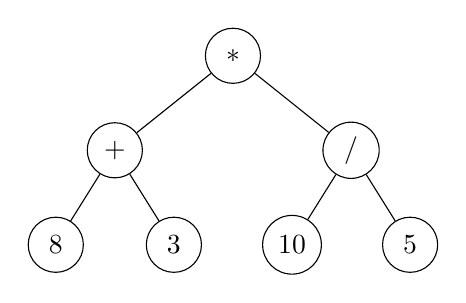
\begin{tikzpicture}[level distance=1.2cm,
  level 1/.style={sibling distance=3cm},
  level 2/.style={sibling distance=1.5cm},
  every node/.style={circle, draw, minimum size=0.7cm}]
\node {$*$}
  child {node {$+$}
    child {node {$8$}}
    child {node {$3$}}
  }
  child {node {$/$}
    child {node {$10$}}
    child {node {$5$}}
  };
\end{tikzpicture}
\end{center}

Lưu ý rằng chúng ta cũng có thể biểu diễn nút lá $8$ dưới dạng $(8, (\varnothing))$. Xét cho cùng, người ta có thể lập luận rằng điều này cũng mô tả một nút không có con nào chứa giá trị. Tuy nhiên, mô tả này mô tả một cây khác. Xét cho cùng, bây giờ nó nói rằng nút $8$ có một con (và do đó là nút trong), nhưng con này không có giá trị (nó là cây rỗng). Để trực quan hóa, một số tác giả đôi khi dùng hình vuông.

Cũng lưu ý rằng giờ chúng ta có thể ``dễ dàng'' định nghĩa cây nhị phân bằng cách đơn giản giới hạn $k = 2$ trong quy tắc Nút trong. Ví dụ $(8, ((3, (\varnothing, (2, \varnothing))), \varnothing))$ sẽ là một cây nhị phân.

Nhưng bạn đã phát hiện ra tác dụng phụ đáng tiếc của định nghĩa này chưa? Trong hình minh họa, cả hình vuông và nút chứa $2$ đều được coi là lá. Xét cho cùng, chúng đều không có con! Do đó, một số sách thay vào đó sử dụng định nghĩa sau cho cây nhị phân. Điều này loại bỏ sự nhập nhằng trong định nghĩa lá, nhưng nhược điểm là không cho phép bất kỳ lá nào có giá trị. Đó là một ví dụ hay về một trong nhiều sự đánh đổi trong khoa học máy tính.

\medskip
\noindent\textbf{Nút lá} $\varnothing \in BTREE$

\noindent\textbf{Nút trong} $(x, (T_1, T_2)) \in BTREE$ nếu $x \in D \land T_1, T_2 \in BTREE$

\noindent\textbf{Tính duy nhất} Không có gì khác thuộc $BTREE$

\medskip
Bây giờ chúng ta đã hình thức hóa định nghĩa cây nhị phân, chúng ta cũng có thể bắt đầu chứng minh các tính chất thú vị về chúng. Một tính chất như vậy là số lá của cây nhị phân $n_L \leq 2^h$ trong đó $h$ là chiều cao của cây. Chứng minh cho khẳng định này giờ có thể theo định dạng quy nạp cấu trúc như đã trình bày ở mục trước:

\begin{proof}
\textbf{Trường hợp cơ sở (Cây rỗng):} Xét quy tắc Cây rỗng của định nghĩa $TREE$. Cây rỗng không có nút nào, nên có chiều cao $0$ và cũng không có lá. Do đó $n_L = 0 \leq 2^0 = 1$ đúng.

\textbf{Trường hợp cơ sở (Nút lá):} Xét quy tắc Nút lá của định nghĩa $TREE$. Một nút lá có chiều cao $0$ vì đường đi dài nhất từ lá đến gốc loại trừ lá không có nút nào (không có nút nào ngoài lá!), do đó $n_L = 1 \leq 2^0 = 1$ đúng.

\textbf{Bước quy nạp (Nút trong):} Cho $T_1$ và $T_2$ là các cây nào đó với $n_{L_1}$ và $n_{L_2}$ là số lá và $h_1$ và $h_2$ là chiều cao tương ứng. Giả sử rằng $n_{L_1} \leq 2^{h_1}$ và $n_{L_2} \leq 2^{h_2}$ (GT quy nạp). Bây giờ dùng quy tắc Nút trong để tạo cây mới $T = (x, (T_1, T_2))$ cho giá trị $x$ nào đó. Với cây $T$ này, $n_L = n_{L_1} + n_{L_2}$ và chiều cao $h = \max(h_1, h_2) + 1$. Bây giờ chúng ta chia trường hợp:

\begin{itemize}
\item $h_1 > h_2$: Trong trường hợp này suy ra $n_{L_2} \leq 2^{h_2} < 2^{h_1}$. Kết quả: $n_L = n_{L_1} + n_{L_2} < 2 \cdot 2^{h_1} = 2^{h_1 + 1} = 2^{\max(h_1, h_2) + 1}$.
\item $h_1 = h_2$: Trong trường hợp này suy ra $n_{L_2} \leq 2^{h_2} = 2^{h_1}$. Kết quả: $n_L = n_{L_1} + n_{L_2} \leq 2 \cdot 2^{h_1} = 2^{h_1 + 1} = 2^{\max(h_1, h_2) + 1}$.
\item $h_1 < h_2$: Tương tự trường hợp đầu.
\end{itemize}

Bây giờ chúng ta đã chỉ ra rằng tính chất đúng cho tất cả các quy tắc của $TREE$ với $k = 2$ trong quy tắc nút trong. Điều này hoàn thành chứng minh bằng quy nạp cấu trúc.
\end{proof}

\subsection*{Bài tập}

\begin{exercise}
Nếu chúng ta không đưa ra giả định rằng $a$, $b$, và $c$ phân biệt, thì tập được ký hiệu bởi $\{a, b, c\}$ thực tế có thể chứa 1, 2, hoặc 3 phần tử. Tập hợp $\{a, b, \{a\}, \{a, c\}, \{a, b, c\}\}$ có thể chứa bao nhiêu phần tử khác nhau? Giải thích câu trả lời của bạn.
\end{exercise}

\begin{exercise}
Tính $A \cup B$, $A \cap B$, và $A \setminus B$ cho mỗi cặp tập hợp sau:
\begin{enumerate}[label=\alph*)]
\item $A = \{a, b, c\}$, $B = \varnothing$
\item $A = \{1, 2, 3, 4, 5\}$, $B = \{2, 4, 6, 8, 10\}$
\item $A = \{a, b\}$, $B = \{a, b, c, d\}$
\item $A = \{a, b, \{a, b\}\}$, $B = \{\{a\}, \{a, b\}\}$
\end{enumerate}
\end{exercise}

\begin{exercise}
Vẽ biểu đồ Venn cho mỗi tập hợp đã tính ở bài tập trước.
\end{exercise}

\begin{exercise}
Nhớ rằng $\mathbb{N}$ biểu diễn tập hợp các số tự nhiên. Nghĩa là, $\mathbb{N} = \{0, 1, 2, 3, \ldots\}$. Cho $X = \{n \in \mathbb{N} \mid n \geq 5\}$, cho $Y = \{n \in \mathbb{N} \mid n \leq 10\}$, và cho $Z = \{n \in \mathbb{N} \mid n \text{ là số chẵn}\}$. Tìm mỗi tập hợp sau:
\begin{enumerate}[label=\alph*)]
\item $X \cap Y$
\item $X \cup Y$
\item $X \setminus Y$
\item $\mathbb{N} \setminus Z$
\item $X \cap Z$
\item $Y \cap Z$
\item $Y \cup Z$
\item $Z \setminus \mathbb{N}$
\end{enumerate}
\end{exercise}

\begin{exercise}
Tìm $\mathcal{P}(\{1, 2, 3\})$. (Gợi ý: Nó có tám phần tử.)
\end{exercise}

\begin{exercise}
Giả sử rằng $a$ và $b$ là các thực thể và $a \neq b$. Cho $A$ và $B$ là các tập được định nghĩa bởi $A = \{a, \{b\}, \{a, b\}\}$ và $B = \{a, b, \{a, \{b\}\}\}$. Xác định mỗi mệnh đề sau đúng hay sai. Giải thích câu trả lời.
\begin{enumerate}[label=\alph*)]
\item $b \in A$
\item $\{a, b\} \subseteq A$
\item $\{a, b\} \subseteq B$
\item $\{a, b\} \in B$
\item $\{a, \{b\}\} \in A$
\item $\{a, \{b\}\} \in B$
\end{enumerate}
\end{exercise}

\begin{exercise}
Vì $\mathcal{P}(A)$ là một tập hợp, nên có thể tạo tập $\mathcal{P}(\mathcal{P}(A))$. $\mathcal{P}(\mathcal{P}(\varnothing))$ là gì? $\mathcal{P}(\mathcal{P}(\{a, b\}))$ là gì? (Gợi ý: Nó có mười sáu phần tử.)
\end{exercise}

\begin{exercise}
Trong câu tiếng Anh ``She likes dogs that are small, cuddly, and cute'' (Cô ấy thích những con chó nhỏ, dễ thương, và đáng yêu), cô ấy thích giao hay hợp của các tập hợp chó? Còn trong câu ``She likes dogs that are small, dogs that are cuddly, and dogs that are cute'' (Cô ấy thích chó nhỏ, chó dễ thương, và chó đáng yêu) thì sao?
\end{exercise}

\begin{exercise}
Nếu $A$ là tập hợp bất kỳ, bạn có thể nói gì về $A \cup A$? Về $A \cap A$? Về $A \setminus A$? Tại sao?
\end{exercise}

\begin{exercise}
Giả sử rằng $A$ và $B$ là các tập hợp sao cho $A \subseteq B$. Bạn có thể nói gì về $A \cup B$? Về $A \cap B$? Về $A \setminus B$? Tại sao?
\end{exercise}

\begin{exercise}
Giả sử rằng $A$, $B$, và $C$ là các tập hợp. Chứng minh rằng $C \subseteq A \cap B$ khi và chỉ khi $(C \subseteq A) \land (C \subseteq B)$.
\end{exercise}

\begin{exercise}
Giả sử rằng $A$, $B$, và $C$ là các tập hợp, và $A \subseteq B$ và $B \subseteq C$. Chứng minh rằng $A \subseteq C$.
\end{exercise}

\begin{exercise}
Giả sử rằng $A$ và $B$ là các tập hợp sao cho $A \subseteq B$. Có nhất thiết đúng rằng $\mathcal{P}(A) \subseteq \mathcal{P}(B)$ không? Tại sao hoặc tại sao không?
\end{exercise}

\begin{exercise}
Cho $M$ là số tự nhiên bất kỳ, và cho $P(n)$ là vị từ có miền diễn giải bao gồm tất cả số tự nhiên lớn hơn hoặc bằng $M$. Giả sử rằng $P(M)$ đúng, và giả sử rằng $P(k) \to P(k+1)$ với mọi $k \geq M$. Chứng minh rằng $P(n)$ đúng với mọi $n \geq M$.
\end{exercise}

\begin{exercise}
Chứng minh rằng số biến mệnh đề luôn nhiều nhất hơn số liên kết đúng một đơn vị cho mọi công thức $\varphi \in PROP$.
\end{exercise}

\begin{exercise}
Cây tam phân là cây trong đó mỗi nút có tối đa ba con. Đưa ra định nghĩa chính thức cây tam phân, và chứng minh định lý về số nút trong cây tam phân.
\end{exercise}


%%%%%%%%%%%%%%%%%%%%%%%%%%%%%%%%%%%%%%%%%%%%%%%%%%%%%
\section{Đại số Bool của tập hợp}
%%%%%%%%%%%%%%%%%%%%%%%%%%%%%%%%%%%%%%%%%%%%%%%%%%%%%

Rõ ràng rằng lý thuyết tập hợp có liên hệ chặt chẽ với logic. Giao và hợp của các tập hợp có thể được định nghĩa theo toán tử logic ``và'' và ``hoặc''. Ký hiệu $\{x \mid P(x)\}$ cho phép sử dụng vị từ để đặc tả tập hợp. Và nếu $A$ là tập hợp bất kỳ, thì công thức $x \in A$ định nghĩa một vị từ một ngôi đúng cho thực thể $x$ khi và chỉ khi $x$ là thành viên của $A$. Vì vậy không nên ngạc nhiên rằng nhiều quy tắc của logic có tương ứng trong lý thuyết tập hợp.

Ví dụ, chúng ta đã lưu ý rằng $\cup$ và $\cap$ là các phép toán giao hoán. Sự kiện này có thể được xác minh bằng các quy tắc logic. Cho $A$ và $B$ là các tập hợp. Theo định nghĩa về sự bằng nhau của tập hợp, chúng ta có thể chứng minh rằng $A \cup B = B \cup A$ bằng cách chỉ ra rằng $\forall x\,((x \in A \cup B) \leftrightarrow (x \in B \cup A))$. Nhưng với mọi $x$,
\begin{align*}
x \in A \cup B &\leftrightarrow x \in A \lor x \in B & &\text{(định nghĩa của } \cup\text{)} \\
&\leftrightarrow x \in B \lor x \in A & &\text{(tính giao hoán của } \lor\text{)} \\
&\leftrightarrow x \in B \cup A & &\text{(định nghĩa của } \cup\text{)}
\end{align*}

Tính giao hoán của $\cap$ suy ra tương tự từ định nghĩa của $\cap$ theo $\land$ và tính giao hoán của $\land$, và lập luận tương tự cho thấy hợp và giao là các phép toán kết hợp.

Các luật phân phối cho logic mệnh đề dẫn đến hai quy tắc tương tự trong lý thuyết tập hợp. Cho $A$, $B$, và $C$ là các tập hợp bất kỳ. Khi đó
\[
A \cup (B \cap C) = (A \cup B) \cap (A \cup C)
\]
và
\[
A \cap (B \cup C) = (A \cap B) \cup (A \cap C)
\]
Các quy tắc này được gọi là \textbf{luật phân phối} cho lý thuyết tập hợp. Để xác minh luật thứ nhất, chúng ta chỉ cần lưu ý rằng với mọi $x$,
\begin{align*}
x \in A \cup (B \cap C) &\leftrightarrow (x \in A) \lor ((x \in B) \land (x \in C)) & &\text{(định nghĩa } \cup, \cap\text{)} \\
&\leftrightarrow ((x \in A) \lor (x \in B)) \land ((x \in A) \lor (x \in C)) & &\text{(phân phối } \lor\text{)} \\
&\leftrightarrow (x \in A \cup B) \land (x \in A \cup C) & &\text{(định nghĩa } \cup\text{)} \\
&\leftrightarrow x \in ((A \cup B) \cap (A \cup C)) & &\text{(định nghĩa } \cap\text{)}
\end{align*}

Luật phân phối thứ hai suy ra theo cách hoàn toàn tương tự.

\subsection{Phần bù tập hợp}

Trong khi $\cup$ tương tự với $\lor$ và $\cap$ tương tự với $\land$, chúng ta chưa thấy phép toán nào trong lý thuyết tập hợp tương tự với toán tử logic ``phủ định'', $\neg$. Cho tập $A$, ta muốn thử định nghĩa $\{x \mid \neg(x \in A)\}$, tập hợp chứa mọi thứ không thuộc $A$. Thật không may, các quy tắc của lý thuyết tập hợp không cho phép chúng ta định nghĩa tập như vậy. Ký hiệu $\{x \mid P(x)\}$ chỉ có thể được dùng khi miền diễn giải của $P$ là một tập hợp, nên phải có tập hợp nền tảng nào đó mà từ đó các phần tử thuộc/không thuộc $A$ được chọn, tức là tập nền tảng nào đó mà $A$ là tập con. Chúng ta có thể vượt qua vấn đề này bằng cách hạn chế thảo luận vào các tập con của một tập cố định nào đó. Tập này được gọi là \textbf{tập vũ trụ}. Hãy nhớ rằng tập vũ trụ chỉ là vũ trụ cho một cuộc thảo luận cụ thể. Nó đơn giản là tập đủ lớn để chứa tất cả các tập đang xét như các tập con. Cho tập vũ trụ $U$ và tập con $A$ bất kỳ của $U$, chúng ta có thể định nghĩa tập $\{x \in U \mid \neg(x \in A)\}$.

\begin{definition}
\label{def:4.1}
Cho $U$ là tập vũ trụ cho trước, và cho $A$ là tập con bất kỳ của $U$. Chúng ta định nghĩa \textbf{phần bù} của $A$ trong $U$ là tập $\overline{A}$ được định nghĩa bởi
\[
\overline{A} = \{x \in U \mid x \notin A\}.
\]
\end{definition}

Thông thường, chúng ta sẽ gọi phần bù của $A$ trong $U$ đơn giản là phần bù của $A$, nhưng bạn nên nhớ rằng bất cứ khi nào phần bù của tập hợp được sử dụng, phải có tập vũ trụ nào đó ở phía sau. Các sách giáo khoa khác có thể dùng $A^c$ để ký hiệu phần bù của $A$.

Cho phép toán phần bù trên tập hợp, chúng ta có thể tìm các tương tự với các quy tắc logic liên quan đến phủ định. Ví dụ, chúng ta biết rằng $p \land \neg p = \mathbb{F}$ với mọi mệnh đề $p$. Suy ra rằng với mọi tập con $A$ của $U$,
\begin{align*}
A \cap \overline{A} &= \{x \in U \mid (x \in A) \land (x \in \overline{A})\} & &\text{(định nghĩa } \cap\text{)} \\
&= \{x \in U \mid (x \in A) \land (x \notin A)\} & &\text{(định nghĩa phần bù)} \\
&= \{x \in U \mid (x \in A) \land \neg(x \in A)\} & &\text{(định nghĩa } \notin\text{)} \\
&= \varnothing
\end{align*}
đẳng thức cuối suy ra vì mệnh đề $(x \in A) \land \neg(x \in A)$ sai với mọi $x$. Tương tự, chúng ta có thể chỉ ra rằng $A \cup \overline{A} = U$ và $\overline{\overline{A}} = A$ (trong đó $\overline{\overline{A}}$ là phần bù của phần bù của $A$, tức là tập có được bằng cách lấy phần bù của $\overline{A}$).

Các luật quan trọng nhất khi làm việc với phần bù tập hợp là \textbf{Luật De Morgan cho tập hợp}. Các luật này, suy ra trực tiếp từ Luật De Morgan cho logic, phát biểu rằng với mọi tập con $A$ và $B$ của tập vũ trụ $U$,
\[
\overline{A \cup B} = \overline{A} \cap \overline{B}
\]
và
\[
\overline{A \cap B} = \overline{A} \cup \overline{B}
\]

Ví dụ, chúng ta có thể xác minh luật thứ nhất bằng phép tính
\begin{align*}
\overline{A \cup B} &= \{x \in U \mid x \notin (A \cup B)\} & &\text{(định nghĩa phần bù)} \\
&= \{x \in U \mid \neg(x \in A \cup B)\} & &\text{(định nghĩa } \notin\text{)} \\
&= \{x \in U \mid \neg(x \in A \lor x \in B)\} & &\text{(định nghĩa } \cup\text{)} \\
&= \{x \in U \mid (\neg(x \in A)) \land (\neg(x \in B))\} & &\text{(Luật De Morgan cho logic)} \\
&= \{x \in U \mid (x \notin A) \land (x \notin B)\} & &\text{(định nghĩa } \notin\text{)} \\
&= \{x \in U \mid (x \in \overline{A}) \land (x \in \overline{B})\} & &\text{(định nghĩa phần bù)} \\
&= \overline{A} \cap \overline{B} & &\text{(định nghĩa } \cap\text{)}
\end{align*}

% Bảng luật Bool
\begin{figure}[ht]
\centering
\begin{tabular}{ll}
\toprule
\textbf{Phần bù kép} & $\overline{\overline{A}} = A$ \\
\midrule
\textbf{Luật hỗn hợp} & $A \cup \overline{A} = U$ \\
& $A \cap \overline{A} = \varnothing$ \\
& $\varnothing \cup A = A$ \\
& $\varnothing \cap A = \varnothing$ \\
\midrule
\textbf{Luật lũy đẳng} & $A \cap A = A$ \\
& $A \cup A = A$ \\
\midrule
\textbf{Luật giao hoán} & $A \cap B = B \cap A$ \\
& $A \cup B = B \cup A$ \\
\midrule
\textbf{Luật kết hợp} & $A \cap (B \cap C) = (A \cap B) \cap C$ \\
& $A \cup (B \cup C) = (A \cup B) \cup C$ \\
\midrule
\textbf{Luật phân phối} & $A \cap (B \cup C) = (A \cap B) \cup (A \cap C)$ \\
& $A \cup (B \cap C) = (A \cup B) \cap (A \cup C)$ \\
\midrule
\textbf{Luật De Morgan} & $\overline{A \cap B} = \overline{A} \cup \overline{B}$ \\
& $\overline{A \cup B} = \overline{A} \cap \overline{B}$ \\
\bottomrule
\end{tabular}
\caption{Một số Luật của Đại số Bool cho tập hợp. $A$, $B$, và $C$ là các tập hợp. Với các luật liên quan đến toán tử phần bù, chúng được giả sử là các tập con của tập vũ trụ $U$. Phần lớn các luật này tương ứng trực tiếp với các luật Đại số Bool cho logic mệnh đề như trong Hình~2.2.}
\label{fig:4.4}
\end{figure}

Một chứng minh quy nạp dễ dàng có thể được dùng để xác minh các phiên bản tổng quát hóa của Luật De Morgan cho lý thuyết tập hợp. (Trong ngữ cảnh này, mọi tập hợp đều được giả sử là tập con của tập vũ trụ không tên nào đó.) Một phép tính đơn giản xác minh Luật De Morgan cho ba tập hợp:
\begin{align*}
\overline{A \cup B \cup C} &= \overline{(A \cup B) \cup C} \\
&= \overline{(A \cup B)} \cap \overline{C} & &\text{(theo Luật De Morgan cho hai tập)} \\
&= (\overline{A} \cap \overline{B}) \cap \overline{C} & &\text{(theo Luật De Morgan cho hai tập)} \\
&= \overline{A} \cap \overline{B} \cap \overline{C}
\end{align*}

Từ đó, chúng ta có thể suy ra các luật tương tự cho bốn tập, năm tập, và vân vân. Tuy nhiên, chỉ nói ``và vân vân'' không phải là chứng minh chặt chẽ. Trong khi chúng ta có thể đã bào chữa cho điều đó ở Chương~2, giờ chúng ta có thể chứng minh sự kiện này. Đây là chứng minh quy nạp chặt chẽ cho Luật De Morgan tổng quát:

\begin{theorem}
\label{thm:4.5}
Với mọi số tự nhiên $n \geq 2$ và với mọi tập hợp $X_1, X_2, \ldots, X_n$,
\[
\overline{X_1 \cup X_2 \cup \cdots \cup X_n} = \overline{X_1} \cap \overline{X_2} \cap \cdots \cap \overline{X_n}
\]
\end{theorem}

\begin{proof}
Chúng ta chứng minh bằng quy nạp. Trong trường hợp cơ sở, $n = 2$, mệnh đề là $\overline{X_1 \cup X_2} = \overline{X_1} \cap \overline{X_2}$. Điều này đúng vì nó chỉ là áp dụng Luật De Morgan cho hai tập hợp.

Cho bước quy nạp, giả sử mệnh đề đúng cho $n = k$. Chúng ta muốn chỉ ra rằng nó đúng cho $n = k + 1$. Cho $X_1, X_2, \ldots, X_{k+1}$ là $k + 1$ tập hợp bất kỳ. Khi đó:
\begin{align*}
\overline{X_1 \cup X_2 \cup \cdots \cup X_{k+1}} &= \overline{(X_1 \cup X_2 \cup \cdots \cup X_k) \cup X_{k+1}} \\
&= \overline{(X_1 \cup X_2 \cup \cdots \cup X_k)} \cap \overline{X_{k+1}} \\
&= (\overline{X_1} \cap \overline{X_2} \cap \cdots \cap \overline{X_k}) \cap \overline{X_{k+1}} \\
&= \overline{X_1} \cap \overline{X_2} \cap \cdots \cap \overline{X_{k+1}}
\end{align*}
Trong phép tính này, bước thứ hai suy ra theo Luật De Morgan cho hai tập, trong khi bước thứ ba suy ra từ giả thiết quy nạp. Do đó theo nguyên lý quy nạp chúng ta đã chứng minh định lý.
\end{proof}

\subsection{Liên hệ giữa logic và lý thuyết tập hợp}

Cũng như các luật logic cho phép chúng ta thực hiện đại số với các công thức logic, các luật lý thuyết tập hợp cho phép chúng ta thực hiện đại số với tập hợp. Vì mối quan hệ chặt chẽ giữa logic và lý thuyết tập hợp, các đại số của chúng rất giống nhau. Đại số của tập hợp, giống như đại số của logic, là \textbf{đại số Bool}. Khi George Boole viết cuốn sách năm 1854 về logic, thực ra nó cũng nói về lý thuyết tập hợp nhiều như logic. Trên thực tế, Boole không phân biệt rõ ràng giữa vị từ và tập hợp các đối tượng mà vị từ đó đúng. Các luật đại số và công thức của ông áp dụng như nhau cho cả hai trường hợp. Chính xác hơn, nếu chúng ta chỉ xét các tập con của tập vũ trụ $U$ cho trước nào đó, thì có sự tương ứng trực tiếp giữa các ký hiệu và phép toán cơ bản của logic mệnh đề và các ký hiệu và phép toán nhất định trong lý thuyết tập hợp, như bảng sau:

\begin{center}
\begin{tabular}{cc}
\toprule
\textbf{Logic} & \textbf{Lý thuyết tập hợp} \\
\midrule
$\mathbb{T}$ & $U$ \\
$\mathbb{F}$ & $\varnothing$ \\
$p \land q$ & $A \cap B$ \\
$p \lor q$ & $A \cup B$ \\
$\neg p$ & $\overline{A}$ \\
\bottomrule
\end{tabular}
\end{center}

Bất kỳ công thức logic hợp lệ hay phép tính nào liên quan đến biến mệnh đề và các ký hiệu $\mathbb{T}$, $\mathbb{F}$, $\land$, $\lor$, và $\neg$ đều có thể được chuyển đổi thành công thức hay phép tính hợp lệ trong lý thuyết tập hợp bằng cách thay các mệnh đề bằng tập con của $U$ và thay các ký hiệu logic bằng $U$, $\varnothing$, $\cap$, $\cup$, và toán tử phần bù. Hình~4.5 minh họa điều này.

Cũng như trong logic, các phép toán lý thuyết tập hợp có thể được kết hợp để tạo các biểu thức phức tạp như $(A \cup C) \cap (B \cup \overline{C} \cup D)$. Dấu ngoặc luôn có thể được dùng trong các biểu thức như vậy để chỉ định thứ tự thực hiện phép toán. Khi không có dấu ngoặc, chúng ta cần quy tắc ưu tiên để xác định thứ tự phép toán. Quy tắc ưu tiên cho đại số Bool của tập hợp được chuyển trực tiếp từ đại số Bool của mệnh đề. Khi hợp và giao được dùng cùng nhau mà không có dấu ngoặc, giao có ưu tiên cao hơn hợp. Hơn nữa, khi nhiều toán tử cùng loại được dùng mà không có dấu ngoặc, chúng được tính từ trái sang phải. (Tất nhiên, vì $\cup$ và $\cap$ đều là phép toán kết hợp, thứ tự tính từ trái sang phải hay phải sang trái không thực sự quan trọng.) Ví dụ, $A \cup B \cap C \cup D$ được tính là $(A \cup (B \cap C)) \cup D$. Phép lấy phần bù là trường hợp đặc biệt. Vì nó được ký hiệu bằng cách vẽ đường gạch trên toán hạng, nên không bao giờ có sự nhập nhằng về phần nào của công thức nó áp dụng.

\begin{warningbox}
Thật không may trong bài viết tay, điều này không phải lúc nào cũng đúng. Hãy đảm bảo viết gọn gàng và rõ ràng khi làm việc với phần bù. Cũng lưu ý rằng, tương tự dấu ngoặc trong logic mệnh đề, mặc dù dấu ngoặc có thể không cần thiết, tôi khuyến khích bạn thêm chúng để cải thiện tính dễ đọc của thứ tự phép toán.
\end{warningbox}

Các luật lý thuyết tập hợp có thể được dùng để đơn giản hóa các biểu thức phức tạp liên quan đến tập hợp. (Như thường lệ, ý nghĩa của ``đơn giản hóa'' phần nào nằm ở người nhìn.) Ví dụ, với mọi tập $X$ và $Y$,
\begin{align*}
(X \cup Y) \cap (Y \cup X) &= (X \cup Y) \cap (X \cup Y) & &\text{(Luật giao hoán)} \\
&= (X \cup Y) & &\text{(Luật lũy đẳng)}
\end{align*}
trong đó ở bước thứ hai, Luật lũy đẳng, nói rằng $A \cap A = A$, được áp dụng với $A = X \cup Y$. Với biểu thức dùng phần bù, thường được coi là đơn giản hơn khi áp dụng phép toán cho từng tập riêng lẻ, như trong $\overline{A}$, thay vì cho công thức, như trong $\overline{A \cap B}$. Luật De Morgan luôn có thể được dùng để đơn giản hóa biểu thức trong đó phần bù được áp dụng cho công thức. Ví dụ,
\begin{align*}
A \cap \overline{B \cup \overline{A}} &= A \cap (\overline{B} \cap \overline{\overline{A}}) & &\text{(Luật De Morgan)} \\
&= A \cap (\overline{B} \cap A) & &\text{(Phần bù kép)} \\
&= A \cap (A \cap \overline{B}) & &\text{(Luật giao hoán)} \\
&= (A \cap A) \cap \overline{B} & &\text{(Luật kết hợp)} \\
&= A \cap \overline{B} & &\text{(Luật lũy đẳng)}
\end{align*}

Như ví dụ cuối cùng về mối quan hệ giữa lý thuyết tập hợp và logic, xét biểu thức lý thuyết tập hợp $A \cap (A \cup B)$ và mệnh đề hợp thành tương ứng $p \land (p \lor q)$. (Chúng tương ứng vì với mọi $x$, $x \in A \cap (A \cup B) \equiv (x \in A) \land ((x \in A) \lor (x \in B))$.) Bạn có thể thấy trực giác rõ ràng rằng $A \cap (A \cup B) = A$. Chính thức, điều này suy ra từ sự kiện rằng $p \land (p \lor q) \equiv p$, có thể kém trực giác hơn và đáng ngạc nhiên là khó chứng minh bằng đại số từ các luật logic. Tuy nhiên, có cách khác để kiểm tra tương đương logic có hợp lệ: Lập bảng chân trị. Xét bảng chân trị cho $p \land (p \lor q)$:

\begin{center}
\begin{tabular}{cc|c|c}
$p$ & $q$ & $p \lor q$ & $p \land (p \lor q)$ \\
\hline
0 & 0 & 0 & 0 \\
0 & 1 & 1 & 0 \\
1 & 0 & 1 & 1 \\
1 & 1 & 1 & 1 \\
\end{tabular}
\end{center}

Sự kiện rằng cột thứ nhất và cột cuối cùng của bảng giống hệt nhau cho thấy $p \land (p \lor q) \equiv p$. Lấy $p$ là mệnh đề $x \in A$ và $q$ là mệnh đề $x \in B$, suy ra rằng các tập $A$ và $A \cap (A \cup B)$ có cùng thành viên và do đó bằng nhau.

\begin{infobox}
Trong một trong các pencast của khóa học, chúng tôi mô tả cách biểu đồ Venn cũng có thể được dùng như các phương án thay thế cho bảng chân trị dựa trên một câu hỏi thi cũ. Bạn có thể tìm pencast đó tại: \url{https://youtu.be/5xle5qfrh0k}.
\end{infobox}

\subsection*{Bài tập}

\begin{exercise}
Sử dụng các luật logic để xác minh các luật kết hợp cho hợp và giao. Nghĩa là, chứng minh rằng nếu $A$, $B$, và $C$ là các tập hợp, thì $A \cup (B \cup C) = (A \cup B) \cup C$ và $A \cap (B \cap C) = (A \cap B) \cap C$.
\end{exercise}

\begin{exercise}
Chứng minh rằng với mọi tập hợp $A$ và $B$, $A \subseteq A \cup B$ và $A \cap B \subseteq A$.
\end{exercise}

\begin{exercise}
Nhớ rằng ký hiệu $\oplus$ biểu thị phép hoặc loại trừ logic. Nếu $A$ và $B$ là các tập hợp, định nghĩa tập $A \triangle B$ bởi $A \triangle B = \{x \mid (x \in A) \oplus (x \in B)\}$. Chứng minh rằng $A \triangle B = (A \setminus B) \cup (B \setminus A)$. ($A \triangle B$ được gọi là \textbf{hiệu đối xứng} của $A$ và $B$.)
\end{exercise}

\begin{exercise}
Chọn ba tập không rỗng $A$, $B$, $C$. Vẽ biểu đồ Venn của $A \triangle B \triangle C$.
\end{exercise}

\begin{exercise}
Cho $A$ là tập con của tập vũ trụ $U$ cho trước. Xác minh rằng $\overline{\overline{A}} = A$ và $A \cup \overline{A} = U$.
\end{exercise}

\begin{exercise}
Xác minh Luật De Morgan thứ hai cho tập hợp, $\overline{A \cap B} = \overline{A} \cup \overline{B}$. Với mỗi bước trong quá trình xác minh, nêu lý do tại sao bước đó hợp lệ.
\end{exercise}

\begin{exercise}
Toán tử tập con, $\subseteq$, được định nghĩa theo toán tử kéo theo logic, $\to$. Tuy nhiên, $\subseteq$ khác với các toán tử $\cap$ và $\cup$ ở chỗ $A \cap B$ và $A \cup B$ là các tập hợp, trong khi $A \subseteq B$ là một mệnh đề. Nên mối quan hệ giữa $\subseteq$ và $\to$ không hoàn toàn giống mối quan hệ giữa $\cup$ và $\lor$ hay giữa $\cap$ và $\land$. Tuy vậy, $\subseteq$ và $\to$ có chung một số tính chất. Bài này cho thấy một ví dụ.
\begin{enumerate}[label=\alph*)]
\item Chứng minh rằng ba mệnh đề hợp thành sau tương đương logic: $p \to q$, $(p \land q) \leftrightarrow p$, và $(p \lor q) \leftrightarrow q$.
\item Chứng minh rằng với mọi tập $A$ và $B$, ba mệnh đề sau tương đương: $A \subseteq B$, $A \cap B = A$, và $A \cup B = B$.
\end{enumerate}
\end{exercise}

\begin{exercise}
Luật De Morgan áp dụng cho các tập con của tập vũ trụ $U$ cho trước. Chứng minh rằng với tập con $X$ của $U$, $\overline{X} = U \setminus X$. Suy ra Luật De Morgan có thể viết là $U \setminus (A \cup B) = (U \setminus A) \cap (U \setminus B)$ và $U \setminus (A \cap B) = (U \setminus A) \cup (U \setminus B)$. Chứng minh rằng các luật này đúng dù $A$ và $B$ có phải tập con của $U$ hay không. Nghĩa là, chứng minh rằng với mọi tập $A$, $B$, và $C$, $C \setminus (A \cup B) = (C \setminus A) \cap (C \setminus B)$ và $C \setminus (A \cap B) = (C \setminus A) \cup (C \setminus B)$.
\end{exercise}

\begin{exercise}
Chứng minh rằng $A \cup (A \cap B) = A$ với mọi tập $A$ và $B$.
\end{exercise}

\begin{exercise}
Cho $X$ và $Y$ là các tập hợp. Đơn giản hóa mỗi biểu thức sau. Giải thích mỗi bước bằng một trong các luật lý thuyết tập hợp.
\begin{enumerate}[label=\alph*)]
\item $X \cup (Y \cup X)$
\item $(X \cap Y) \cap \overline{X}$
\item $(X \cup Y) \cap \overline{Y}$
\item $(X \cup Y) \cup (X \cap Y)$
\end{enumerate}
\end{exercise}

\begin{exercise}
Cho $A$, $B$, và $C$ là các tập hợp. Đơn giản hóa mỗi biểu thức sau. Trong câu trả lời, toán tử phần bù chỉ nên áp dụng cho từng tập riêng lẻ $A$, $B$, và $C$.
\begin{enumerate}[label=\alph*)]
\item $\overline{A \cup B \cup C}$
\item $\overline{A \cup (\overline{B \cap C})}$
\item $\overline{A \cup B}$
\item $\overline{B \cap \overline{C}}$
\item $\overline{A \cap B \cap C}$
\item $A \cap \overline{A \cup B}$
\end{enumerate}
\end{exercise}

\begin{exercise}
Sử dụng quy nạp để chứng minh Luật De Morgan tổng quát sau cho lý thuyết tập hợp: Với mọi số tự nhiên $n \geq 2$ và với mọi tập $X_1, X_2, \ldots, X_n$,
\[
\overline{X_1 \cap X_2 \cap \cdots \cap X_n} = \overline{X_1} \cup \overline{X_2} \cup \cdots \cup \overline{X_n}
\]
\end{exercise}

\begin{exercise}
Phát biểu và chứng minh các luật phân phối tổng quát cho lý thuyết tập hợp.
\end{exercise}


%%%%%%%%%%%%%%%%%%%%%%%%%%%%%%%%%%%%%%%%%%%%%%%%%%%%%
\section{Ứng dụng: Đồ thị}
%%%%%%%%%%%%%%%%%%%%%%%%%%%%%%%%%%%%%%%%%%%%%%%%%%%%%

Tổng quát hóa từ cấu trúc dữ liệu cây, chúng ta có thể tạo \textbf{đồ thị}. Trong khoa học máy tính, chúng ta có thể mô hình hóa nhiều bài toán khác nhau dưới dạng đồ thị: từ đường đi ngắn nhất để hỗ trợ hệ thống định vị, đến lập lịch các trận đấu thể thao. Hãy nghĩ về đồ thị giống như cây, ngoại trừ việc có thể có cạnh giữa các nút ``anh em'' --- và hơn thế nữa.

\subsection{Thuật ngữ đồ thị}

Đồ thị là một bộ 2 gồm hai tập hợp thường được ký hiệu $G = (V, E)$. Tọa độ thứ nhất $V$ là tập hợp các \textbf{đỉnh}, còn gọi là các \textbf{nút}. Tọa độ thứ hai $E$ là tập hợp các \textbf{cạnh}, trong đó mỗi cạnh biểu diễn một kết nối giữa hai đỉnh. Hai đỉnh được nối bởi một cạnh được gọi là \textbf{láng giềng}. Về mặt đồ họa, chúng ta thường vẽ các đỉnh dưới dạng hình tròn và các cạnh dưới dạng đường nối giữa chúng, giống như chúng ta đã làm với cây ở chương trước. Ví dụ xét biểu diễn trực quan sau của đồ thị $G_1$:

\begin{center}
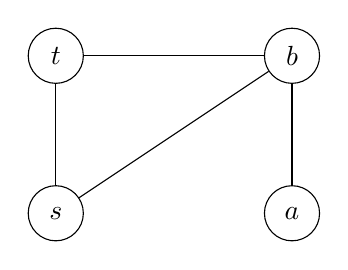
\begin{tikzpicture}[every node/.style={circle, draw, minimum size=0.7cm}]
\node (s) at (0,0) {$s$};
\node (a) at (3,0) {$a$};
\node (t) at (0,2) {$t$};
\node (b) at (3,2) {$b$};
\draw (s) -- (t);
\draw (s) -- (b);
\draw (a) -- (b);
\draw (b) -- (t);
\end{tikzpicture}
\end{center}

Đồ thị này cũng có thể được biểu diễn chính thức hơn:
\[
G_1 = (\{s, a, b, t\}, \{\{s, t\}, \{s, b\}, \{a, b\}, \{b, t\}\})
\]

Đồ thị này là cái chúng ta gọi là \textbf{vô hướng}, nghĩa là các cạnh không có hướng. Do đó chúng ta biểu diễn các cạnh dưới dạng tập hợp, có nghĩa là $E \subseteq \{\{v_1, v_2\} \mid v_1 \neq v_2 \land v_1, v_2 \in V\}$. Ngược lại, trong \textbf{đồ thị có hướng}, các cạnh có gốc và đích. Xét đồ thị $G_2$:

\begin{center}
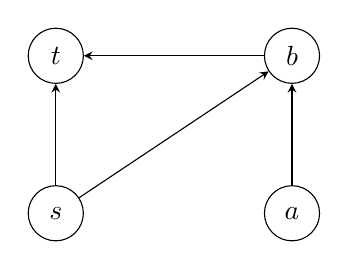
\begin{tikzpicture}[every node/.style={circle, draw, minimum size=0.7cm},
                    >=stealth, ->]
\node (s) at (0,0) {$s$};
\node (a) at (3,0) {$a$};
\node (t) at (0,2) {$t$};
\node (b) at (3,2) {$b$};
\draw (s) -> (t);
\draw (s) -> (b);
\draw (a) -> (b);
\draw (b) -> (t);
\end{tikzpicture}
\end{center}

Đồ thị này có thể được biểu diễn dưới dạng bộ 2:
\[
G_2 = (\{s, a, b, t\}, \{(s, t), (s, b), (a, b), (b, t)\})
\]

Lưu ý rằng với đồ thị có hướng, $E \subseteq V \times V$. Cuối cùng, chúng ta định nghĩa \textbf{đường đi} là một dãy các cạnh. Ví dụ đường đi $\pi = ((s, b), (b, t))$ biểu thị đường đi từ $s$ đến $t$ trong đồ thị $G_2$ ở trên.

Trong Mục~4.5.5 chúng ta sẽ xem lại mô hình đồ thị này và khám phá xem việc bổ sung hàm có thể làm gì để làm phong phú mô hình đồ thị.

\subsection{Ứng dụng đồ thị: Sắp xếp công việc}

Khi bạn đang học môn \textit{Lập luận \& Logic}, bạn có nhiều công việc khác nhau cần hoàn thành. Đọc các phần trong sách, làm bài tập trong sách, bài tập về nhà, và tất nhiên các kỳ thi. Điều này có thể khá choáng ngợp, cả trong việc tìm ra nơi bắt đầu, cũng như tìm ra thứ tự hoàn thành công việc. May mắn thay, bạn có thể dùng đồ thị để giúp cấu trúc các công việc!

Nếu bạn được cho một số công việc cần làm, với các ràng buộc thứ tự giữa chúng (ví dụ bạn cần đọc sách và xem video, trước khi làm bài tập) dưới dạng tập hợp các cặp có thứ tự. Bạn có thể mô hình hóa bài toán này dưới dạng đồ thị, biến các công việc thành đỉnh và các ràng buộc thứ tự thành cạnh. Kết quả có thể trông rất giống những gì bạn thấy trên ad-cs.ewi.tudelft.nl! Giả sử rằng có thể hoàn thành các công việc, đồ thị của bạn sẽ là cái mà chúng ta gọi là \textbf{Đồ thị Có hướng Không chu trình} (hay \textbf{DAG}). Xét cho cùng, nếu có chu trình nào đó trong đồ thị, thì không bao giờ hoàn thành được công việc! (Bạn thấy tại sao không?)

Bây giờ để tìm thứ tự mà các công việc có thể được hoàn thành, chúng ta tìm cái gọi là \textbf{sắp xếp tôpô}. Trong một sắp xếp như vậy, chúng ta đánh số các đỉnh $v_1$ đến $v_{|V|}$ sao cho với mọi cạnh $(v_x, v_y) \in E$, ta có $x < y$. Ví dụ, với đồ thị $G_2$ ở mục trước, $a, s, b, t$ là một sắp xếp tôpô khả thi. Phương pháp tìm sắp xếp tôpô như sau:

\begin{enumerate}
\item Chọn một đỉnh không có cạnh đến.
\item Thêm nó vào sắp xếp tôpô, và loại bỏ nó cùng các cạnh đi của nó khỏi đồ thị.
\item Khi vẫn còn đỉnh, quay lại bước 1.
\end{enumerate}

Trong bài tập, bạn sẽ được yêu cầu viết chứng minh bằng phản chứng để chứng minh rằng luôn tồn tại đỉnh không có cạnh đến trong DAG. Bạn sẽ phân tích thêm và cũng cài đặt thuật toán này trong môn \textit{Thuật toán \& Cấu trúc Dữ liệu}.

\subsection*{Bài tập}

\begin{exercise}
Vẽ đồ thị vô hướng gồm 10 đỉnh, sao cho đường đi dài nhất trong đồ thị gồm 6 cạnh.
\end{exercise}

\begin{exercise}
Vẽ đồ thị có hướng không chu trình gồm 8 đỉnh và 13 cạnh.
\end{exercise}

\begin{exercise}
Đưa ra sắp xếp tôpô của DAG bạn đã vẽ ở bài trước.
\end{exercise}

\begin{exercise}
Chứng minh khẳng định sau: ``Mọi DAG đều có ít nhất một đỉnh không có cạnh đến.'' Bạn có thể thấy chứng minh bằng phản chứng hữu ích ở đây.
\end{exercise}


%%%%%%%%%%%%%%%%%%%%%%%%%%%%%%%%%%%%%%%%%%%%%%%%%%%%%
\section{Ứng dụng: Lập trình với Tập hợp}
%%%%%%%%%%%%%%%%%%%%%%%%%%%%%%%%%%%%%%%%%%%%%%%%%%%%%

Trên máy tính, mọi dữ liệu cuối cùng đều được biểu diễn dưới dạng chuỗi số không và số một. Đôi khi, máy tính cần làm việc với tập hợp. Làm thế nào tập hợp có thể được biểu diễn dưới dạng chuỗi số không và số một? Và một khi đã biểu diễn tập hợp trên máy tính, chúng ta lập trình với chúng như thế nào?

\begin{warningbox}
Trong mục này chúng ta đi vào chi tiết về biểu diễn và tính toán với tập hợp. Bạn sẽ không bị kiểm tra về nội dung này trong môn \textit{Lập luận \& Logic}. Bạn sẽ thấy rằng có khá nhiều phần chồng lấn với tài liệu học môn \textit{Tổ chức Máy tính}, khi chúng ta thảo luận về các hệ thống số khác nhau.
\end{warningbox}

\subsection{Biểu diễn tập hợp}

Tập hợp được xác định bởi các phần tử của nó. Cho tập $A$ và thực thể $x$, câu hỏi cơ bản là: $x$ có thuộc $A$ hay không? Nếu chúng ta biết câu trả lời cho câu hỏi này với mọi $x$ có thể, thì chúng ta biết tập hợp. Với $x$ cho trước, câu trả lời cho câu hỏi ``$x$ có phải thành viên của $A$ không'' là có hoặc không. Câu trả lời có thể được mã hóa bằng cách cho $1$ đại diện cho có và $0$ đại diện cho không. Câu trả lời, khi đó, là một \textbf{bit} đơn, nghĩa là giá trị có thể là không hoặc một. Để biểu diễn tập $A$ dưới dạng chuỗi số không và số một, chúng ta có thể dùng một bit cho mỗi phần tử có thể của $A$. Nếu phần tử $x$ có thể nằm trong tập, thì bit tương ứng có giá trị một. Nếu $x$ không thuộc tập, thì bit tương ứng có giá trị không.

Trong trường hợp số phần tử có thể của tập rất lớn hoặc vô hạn, việc biểu diễn tập theo cách này không khả thi. Nó sẽ đòi hỏi quá nhiều bit, có thể vô hạn. Trong trường hợp đó, biểu diễn khác cho tập có thể được dùng. Tuy nhiên, giả sử chúng ta chỉ quan tâm đến các tập con của tập nhỏ cho trước nào đó. Vì tập này đóng vai trò tập vũ trụ, gọi nó là $U$. Để biểu diễn tập con của $U$, chúng ta chỉ cần một bit cho mỗi thành viên của $U$. Nếu số thành viên của $U$ là $n$, thì tập con của $U$ được biểu diễn bởi chuỗi $n$ số không và một. Hơn nữa, mọi chuỗi $n$ số không và một xác định một tập con của $U$, cụ thể là tập con chứa đúng các phần tử của $U$ tương ứng với số một trong chuỗi. Bạn đã biết từ môn \textit{Tổ chức Máy tính} rằng chuỗi $n$ số không và một được gọi là \textbf{số nhị phân $n$-bit}. Vậy, nếu $U$ là tập có $n$ phần tử, thì các tập con của $U$ tương ứng với các số nhị phân $n$-bit.

Để cụ thể hơn, cho $U$ là tập $\{0, 1, 2, \ldots, 31\}$. Tập này gồm 32 số nguyên từ 0 đến 31. Khi đó mỗi tập con của $U$ có thể được biểu diễn bởi số nhị phân 32-bit. Chúng ta dùng 32 bit vì hầu hết ngôn ngữ lập trình có thể làm việc trực tiếp với số 32-bit. Ví dụ, ngôn ngữ lập trình Java có kiểu dữ liệu \texttt{int}. Giá trị kiểu \texttt{int} là số nhị phân 32-bit.\footnote{Nếu trong phiên bản Java tương lai, giá trị kiểu \texttt{int} là số 64-bit --- có thể dùng để biểu diễn tập con của $\{0, 1, 2, \ldots, 63\}$ --- nguyên lý vẫn như nhau.} Trước khi có tương ứng xác định giữa tập con của $U$ và số 32-bit, chúng ta phải quyết định bit nào trong số sẽ tương ứng với phần tử nào của $U$. Theo truyền thống, chúng ta giả sử rằng các bit được đánh số từ phải sang trái. Nghĩa là, bit ngoài cùng bên phải tương ứng với phần tử $0$ trong $U$, bit thứ hai từ phải tương ứng với $1$, bit thứ ba từ phải tương ứng với $2$, v.v. Ví dụ, số nhị phân 32-bit
\[
1000000000000000000001001110110
\]
tương ứng với tập con $\{1, 2, 4, 5, 6, 9, 31\}$. Vì bit ngoài cùng bên trái là $1$, số $31$ thuộc tập; vì bit tiếp theo là $0$, số $30$ không thuộc tập; và cứ thế.

Từ bây giờ, tôi sẽ viết số nhị phân với chỉ số dưới $2$ để tránh nhầm lẫn với số thường. Hơn nữa, chúng ta sẽ thường bỏ các số không ở đầu. Ví dụ, $1101_2$ là số nhị phân được viết đầy đủ là
\[
00000000000000000000000000001101
\]
và tương ứng với tập $\{0, 2, 3\}$. Mặt khác $1101$ biểu diễn số thường một nghìn một trăm lẻ một.

Ngay cả với ký hiệu này, việc viết ra các số nhị phân dài có thể rất phiền --- và gần như không thể đọc được. Nên số nhị phân không bao giờ được viết dưới dạng chuỗi số không và một trong chương trình máy tính. Một giải pháp thay thế là dùng \textbf{số thập lục phân}. Số thập lục phân được viết bằng mười sáu ký hiệu 0, 1, 2, 3, 4, 5, 6, 7, 8, 9, A, B, C, D, E, và F. Các ký hiệu này được gọi là \textbf{chữ số thập lục phân}. Mỗi chữ số thập lục phân tương ứng với số nhị phân 4-bit, như bảng sau.

\begin{figure}[ht]
\centering
\begin{tabular}{cc|cc}
\toprule
\textbf{Hex.} & \textbf{Nhị phân} & \textbf{Hex.} & \textbf{Nhị phân} \\
\midrule
0 & $0000_2$ & 8 & $1000_2$ \\
1 & $0001_2$ & 9 & $1001_2$ \\
2 & $0010_2$ & A & $1010_2$ \\
3 & $0011_2$ & B & $1011_2$ \\
4 & $0100_2$ & C & $1100_2$ \\
5 & $0101_2$ & D & $1101_2$ \\
6 & $0110_2$ & E & $1110_2$ \\
7 & $0111_2$ & F & $1111_2$ \\
\bottomrule
\end{tabular}
\caption{16 chữ số thập lục phân và các số nhị phân tương ứng. Mỗi chữ số thập lục phân tương ứng với số nhị phân 4-bit. Số nhị phân dài hơn có thể được viết bằng hai hoặc nhiều chữ số thập lục phân. Ví dụ, $101000011111_2 = \texttt{0xA1F}$.}
\label{fig:4.6}
\end{figure}

Để biểu diễn số nhị phân dài hơn, nhiều chữ số thập lục phân có thể được nối lại. Ví dụ, số thập lục phân C7 biểu diễn số nhị phân $11000111_2$. Trong Java và nhiều ngôn ngữ liên quan, số thập lục phân được viết với tiền tố \texttt{0x}. Vậy, số thập lục phân C7 sẽ xuất hiện trong chương trình là \texttt{0xC7}. Chúng ta sẽ theo cùng quy ước ở đây. Bất kỳ số nhị phân 32-bit nào cũng có thể viết bằng tám chữ số thập lục phân (hoặc ít hơn nếu bỏ số không ở đầu). Vậy, các tập con của $\{0, 1, 2, \ldots, 31\}$ tương ứng với số thập lục phân 8 chữ số. Ví dụ, tập con $\{1, 2, 4, 5, 6, 9, 31\}$ tương ứng với \texttt{0x80000276}, biểu diễn số nhị phân $10000000000000000000010011101110_2$. Tương tự, \texttt{0xFF} tương ứng với $\{0, 1, 2, 3, 4, 5, 6, 7\}$ và \texttt{0x1101} tương ứng với số nhị phân $0001000100000001_2$ và tập $\{0, 8, 12\}$.

Bây giờ, nếu bạn đã làm việc với số nhị phân hoặc số thập lục phân, bạn biết rằng chúng có một cách diễn giải khác, phổ biến hơn. Chúng biểu diễn các số nguyên thường. Cũng như $342$ biểu diễn số nguyên $3 \cdot 10^2 + 4 \cdot 10^1 + 2 \cdot 10^0$, số nhị phân $1101_2$ biểu diễn số nguyên $1 \cdot 2^3 + 1 \cdot 2^2 + 0 \cdot 2^1 + 1 \cdot 2^0$, hay $13$. Khi dùng theo cách này, số nhị phân được gọi là số \textbf{cơ số 2}, cũng như số thường là số cơ số 10. Số thập lục phân có thể được diễn giải là số cơ số 16. Ví dụ, \texttt{0x3C7} biểu diễn số nguyên $3 \cdot 16^2 + 12 \cdot 16^1 + 7 \cdot 16^0$, hay $967$. Vậy, $1101_2$ thực sự biểu diễn số nguyên $13$, hay biểu diễn tập $\{0, 2, 3\}$? Câu trả lời là đối với con người, $1101_2$ có thể biểu diễn cả hai. Cả hai đều là diễn giải hợp lệ, và câu hỏi thực sự duy nhất là diễn giải nào hữu ích trong hoàn cảnh cụ thể. Mặt khác, đối với máy tính, $1101_2$ không biểu diễn bất cứ thứ gì. Nó chỉ là chuỗi bit, và máy tính thao tác các bit theo chương trình, mà không quan tâm đến diễn giải.

Tất nhiên, chúng ta vẫn phải trả lời câu hỏi liệu có bao giờ hữu ích khi diễn giải chuỗi bit trong máy tính là biểu diễn tập hợp hay không.

\subsection{Tính toán với tập hợp}

Nếu tất cả những gì chúng ta có thể làm với tập hợp chỉ là ``biểu diễn'' chúng, thì không hữu ích lắm. Chúng ta cần có khả năng tính toán với tập hợp. Nghĩa là, chúng ta cần thực hiện được các phép toán tập hợp như hợp và phần bù.

Nhiều ngôn ngữ lập trình cung cấp các toán tử thực hiện phép toán tập hợp. Trong Java và các ngôn ngữ liên quan, các toán tử thực hiện hợp, giao, và phần bù được viết là \texttt{|}, \texttt{\&}, và \texttt{\~{}}. Ví dụ, nếu \texttt{x} và \texttt{y} là số nguyên 32-bit biểu diễn hai tập con $X$ và $Y$ của $\{0, 1, 2, \ldots, 31\}$, thì \texttt{x | y} là số nguyên 32-bit biểu diễn tập $X \cup Y$. Tương tự, \texttt{x \& y} biểu diễn tập $X \cap Y$, và \texttt{\~{}x} biểu diễn phần bù $\overline{X}$.

Các toán tử \texttt{|}, \texttt{\&}, và \texttt{\~{}} được gọi là \textbf{toán tử logic theo bit} vì cách chúng hoạt động trên từng bit riêng lẻ của các số mà chúng áp dụng. Nếu $0$ và $1$ được diễn giải là giá trị logic sai và đúng, thì các toán tử logic theo bit thực hiện các phép toán logic $\lor$, $\land$, và $\neg$ trên từng bit riêng lẻ. Để thấy tại sao điều này đúng, hãy xem các phép tính mà các toán tử này phải thực hiện.

Cho $k$ là một trong các phần tử của $\{0, 1, 2, \ldots, 31\}$. Trong các số nhị phân \texttt{x}, \texttt{y}, \texttt{x | y}, \texttt{x \& y}, và \texttt{\~{}x}, số $k$ tương ứng với bit ở vị trí $k$. Nghĩa là, $k$ thuộc tập được biểu diễn bởi số nhị phân khi và chỉ khi bit ở vị trí $k$ trong số nhị phân đó là $1$. Xét như tập hợp, \texttt{x \& y} là giao của \texttt{x} và \texttt{y}, nên $k$ là thành viên của tập biểu diễn bởi \texttt{x \& y} khi và chỉ khi $k$ là thành viên của cả hai tập biểu diễn bởi \texttt{x} và \texttt{y}. Nghĩa là, bit $k$ là $1$ trong số nhị phân \texttt{x \& y} khi và chỉ khi bit $k$ là $1$ trong \texttt{x} và bit $k$ là $1$ trong \texttt{y}. Khi diễn giải $1$ là đúng và $0$ là sai, chúng ta thấy rằng bit $k$ của \texttt{x \& y} được tính bằng cách áp dụng toán tử logic ``và'', $\land$, cho bit $k$ của \texttt{x} và bit $k$ của \texttt{y}. Tương tự, bit $k$ của \texttt{x | y} được tính bằng cách áp dụng toán tử logic ``hoặc'', $\lor$, cho bit $k$ của \texttt{x} và bit $k$ của \texttt{y}. Và bit $k$ của \texttt{\~{}x} được tính bằng cách áp dụng toán tử logic ``phủ định'', $\neg$, cho bit $k$ của \texttt{x}. Trong mỗi trường hợp, toán tử logic được áp dụng cho từng vị trí bit riêng biệt. (Tất nhiên, thảo luận này chỉ là dịch sang ngôn ngữ bit của các định nghĩa phép toán tập hợp theo toán tử logic: $A \cap B = \{x \mid x \in A \land x \in B\}$, $A \cup B = \{x \mid x \in A \lor x \in B\}$, và $\overline{A} = \{x \in U \mid \neg(x \in A)\}$.)

Ví dụ, xét các số nhị phân $1011010_2$ và $10111_2$, biểu diễn các tập $\{1, 3, 4, 6\}$ và $\{0, 1, 2, 4\}$. Khi đó $1011010_2$ \texttt{\&} $10111_2$ là $10010_2$. Số nhị phân này biểu diễn tập $\{1, 4\}$, chính là giao $\{1, 3, 4, 6\} \cap \{0, 1, 2, 4\}$. Dễ thấy hơn nếu viết phép tính theo cột:

\begin{center}
\begin{tabular}{r@{\quad}l}
 & $1011010 \quad \{6,\; 4,\; 3,\; 1\}$ \\
\texttt{\&} & $0010111 \quad \{4,\; 2,\; 1,\; 0\}$ \\
\hline
 & $0010010 \quad \{4,\; 1\}$ \\
\end{tabular}
\end{center}

Lưu ý rằng trong mỗi cột của số nhị phân, bit ở hàng dưới được tính là ``và'' logic của hai bit nằm phía trên nó. Tương tự, hợp của hai tập được tính bằng ``hoặc'' theo bit:

\begin{center}
\begin{tabular}{r@{\quad}l}
 & $1011010 \quad \{6,\; 4,\; 3,\; 1\}$ \\
\texttt{|} & $0010111 \quad \{4,\; 2,\; 1,\; 0\}$ \\
\hline
 & $1011111 \quad \{6,\; 4,\; 3,\; 2,\; 1,\; 0\}$ \\
\end{tabular}
\end{center}

Phần bù của tập được tính bằng phép ``phủ định'' theo bit. Vì chúng ta đang làm việc với số nhị phân 32-bit, phần bù được lấy theo tập vũ trụ $\{0, 1, 2, \ldots, 31\}$. Vậy ví dụ,
\[
\texttt{\~{}}1011010_2 = 11111111111111111111111101001012
\]

Tất nhiên, chúng ta có thể áp dụng các toán tử \texttt{\&}, \texttt{|}, và \texttt{\~{}} cho số viết ở dạng thập lục phân, hay thậm chí dạng thường cơ số 10. Khi tính bằng tay, tốt nhất là chuyển số sang dạng nhị phân. Ví dụ,
\begin{align*}
\texttt{0xAB7} \;\texttt{\&}\; \texttt{0x168E} &= 1010\;1011\;0111_2 \;\texttt{\&}\; 1\;0110\;1000\;1110_2 \\
&= 0\;0010\;1000\;0110_2 \\
&= \texttt{0x286}
\end{align*}

Khi tính toán với tập hợp, đôi khi cần làm việc với từng phần tử riêng lẻ. Các thao tác điển hình bao gồm thêm phần tử vào tập, loại bỏ phần tử khỏi tập, và kiểm tra phần tử có thuộc tập hay không. Tuy nhiên, thay vì làm việc với phần tử trực tiếp, thuận tiện hơn khi làm việc với tập chỉ chứa phần tử đó. Ví dụ, kiểm tra $5 \in A$ giống như kiểm tra $\{5\} \cap A \neq \varnothing$. Tập $\{5\}$ được biểu diễn bởi số nhị phân $100000_2$ hay số thập lục phân \texttt{0x20}. Giả sử tập $A$ được biểu diễn bởi số \texttt{x}. Khi đó, kiểm tra $5 \in A$ tương đương với kiểm tra \texttt{0x20 \& x} $\neq$ \texttt{0}. Tương tự, tập $A \cup \{5\}$, có được bằng cách thêm $5$ vào $A$, có thể tính là \texttt{x | 0x20}. Tập $A \setminus \{5\}$, là tập có được bằng cách loại $5$ khỏi $A$ nếu nó có trong $A$, được biểu diễn bởi \texttt{x \& \~{}0x20}.

Các tập $\{0\}, \{1\}, \{2\}, \{3\}, \{4\}, \{5\}, \{6\}, \ldots, \{31\}$ được biểu diễn bởi các số thập lục phân \texttt{0x1}, \texttt{0x2}, \texttt{0x4}, \texttt{0x8}, \texttt{0x10}, \texttt{0x20}, \ldots, \texttt{0x80000000}. Trong các ứng dụng máy tính thực tế, một số trong các số này được đặt tên, và các tên này được coi là tên cho các phần tử có thể của tập (mặc dù, nói đúng ra, chúng là tên cho các tập chứa các phần tử đó). Giả sử, ví dụ, \texttt{a}, \texttt{b}, \texttt{c}, và \texttt{d} là tên cho bốn trong số các số từ danh sách trên. Khi đó \texttt{a | c} là tập chứa hai phần tử tương ứng với \texttt{a} và \texttt{c}. Nếu \texttt{x} là tập, thì \texttt{x \& \~{}d} là tập có được bằng cách loại \texttt{d} khỏi \texttt{x}. Và chúng ta có thể kiểm tra \texttt{b} có thuộc \texttt{x} hay không bằng cách kiểm tra \texttt{x \& b} $\neq$ \texttt{0}.

Đây là ví dụ thực tế, được dùng trong hệ điều hành Apple Mac (macOS). Ký tự có thể được in hay hiển thị trên màn hình với nhiều kích cỡ và kiểu dáng khác nhau. \textbf{Phông chữ} là bộ sưu tập hình ảnh ký tự với kích cỡ và kiểu dáng cụ thể. Trên Mac, phông chữ cơ bản có thể được sửa đổi bằng cách chỉ định bất kỳ thuộc tính kiểu dáng nào sau: \textit{bold}, \textit{italic}, \textit{underline}, \textit{outline}, \textit{shadow}, \textit{condense}, và \textit{extend}. Kiểu dáng của phông chữ là tập con của tập các thuộc tính này. Tập kiểu dáng có thể được chỉ định bằng cách or các thuộc tính riêng lẻ. Ví dụ, phông chữ gạch chân, in đậm, nghiêng có tập kiểu dáng \texttt{underline | bold | italic}. Với phông chữ thường, không có thuộc tính kiểu dáng nào, tập kiểu dáng là tập rỗng, biểu diễn bởi số không.

Ngôn ngữ lập trình Java dùng sơ đồ tương tự để chỉ định thuộc tính kiểu dáng cho phông chữ, nhưng hiện tại chỉ có hai thuộc tính cơ bản, \texttt{Font.BOLD} và \texttt{Font.ITALIC}. Ví dụ thú vị hơn trong Java được cung cấp bởi các loại sự kiện. Sự kiện trong Java biểu diễn một số loại hành động người dùng, như nhấn phím trên bàn phím. Sự kiện được liên kết với ``thành phần'' như cửa sổ, nút và thanh cuộn. Thành phần có thể được đặt để bỏ qua loại sự kiện cho trước. Khi đó chúng ta nói rằng loại sự kiện đó bị \textit{tắt} cho thành phần đó. Nếu thành phần được đặt để xử lý sự kiện của loại cho trước, thì loại sự kiện đó được nói là \textit{bật}. Mỗi thành phần theo dõi tập các loại sự kiện hiện đang bật. Nó sẽ bỏ qua bất kỳ sự kiện nào có loại không thuộc tập đó. Mỗi loại sự kiện có hằng số liên kết với tên như \texttt{AWTEvent.MOUSE\_EVENT\_MASK}. Các hằng số này biểu diễn các phần tử có thể của tập loại sự kiện. Tập loại sự kiện có thể được chỉ định bằng cách or nhiều hằng số như vậy. Nếu \texttt{c} là thành phần và \texttt{x} là số biểu diễn tập loại sự kiện, thì lệnh `\texttt{c.enableEvents(x)}' bật các sự kiện trong tập \texttt{x} cho thành phần \texttt{c}. Nếu \texttt{y} biểu diễn tập loại sự kiện đã bật cho \texttt{c}, thì hiệu ứng của lệnh này là thay \texttt{y} bằng hợp \texttt{y | x}. Lệnh khác, `\texttt{c.disableEvents(x)}', sẽ tắt các loại sự kiện trong \texttt{x} cho thành phần \texttt{c}. Nó thực hiện điều này bằng cách thay tập hiện tại \texttt{y} bằng \texttt{y \& \~{}x}.

\subsection*{Bài tập}

\begin{exercise}
Giả sử số \texttt{x} và \texttt{y} biểu diễn các tập $A$ và $B$. Chứng minh rằng tập $A \setminus B$ được biểu diễn bởi \texttt{x \& (\~{}y)}.
\end{exercise}

\begin{exercise}
Viết mỗi số nhị phân sau ở dạng thập lục phân:
\begin{enumerate}[label=\alph*)]
\item $10110110_2$
\item $10_2$
\item $111100001111_2$
\item $101001_2$
\end{enumerate}
\end{exercise}

\begin{exercise}
Viết mỗi số thập lục phân sau ở dạng nhị phân:
\begin{enumerate}[label=\alph*)]
\item \texttt{0x123}
\item \texttt{0xFADE}
\item \texttt{0x137F}
\item \texttt{0xFF11}
\end{enumerate}
\end{exercise}

\begin{exercise}
Cho giá trị mỗi biểu thức sau dưới dạng số thập lục phân:
\begin{enumerate}[label=\alph*)]
\item \texttt{0x73 | 0x56A}
\item \texttt{\~{}0x3FF0A2FF}
\item \texttt{(0x44 | 0x95) \& 0xE7}
\item \texttt{0x5C35A7 \& 0xFF00}
\item \texttt{0x5C35A7 \& \~{}0xFF00}
\item \texttt{\~{}(0x1234 \& 0x4321)}
\end{enumerate}
\end{exercise}

\begin{exercise}
Tìm máy tính (hoặc chương trình máy tính trên máy tính) có thể làm việc với số thập lục phân. Viết báo cáo ngắn giải thích cách làm việc với số thập lục phân trên máy tính đó. Đặc biệt giải thích cách dùng máy tính để giải bài trước.
\end{exercise}

\begin{exercise}
Câu hỏi này giả sử bạn biết cách cộng số nhị phân. Giả sử \texttt{x} và \texttt{y} là số nhị phân. Trong trường hợp nào các số nhị phân \texttt{x + y} và \texttt{x | y} giống nhau?
\end{exercise}

\begin{exercise}
Ngoài số thập lục phân, các ngôn ngữ lập trình Java và C (nhưng không phải phiên bản mới nhất của C++) hỗ trợ số bát phân. Tìm hiểu và báo cáo về số bát phân trong Java hoặc C. Giải thích số bát phân là gì, cách viết, và cách sử dụng.
\end{exercise}

\begin{exercise}
Trong hệ điều hành Unix (và Linux, macOS, \ldots), mỗi tệp có tập quyền liên kết, xác định ai có thể dùng tệp và cách sử dụng. Tập quyền cho tệp cho trước được biểu diễn bởi số nhị phân chín bit. Số này đôi khi được viết dưới dạng số bát phân. Tìm hiểu và báo cáo về hệ thống quyền Unix. Tập quyền nào được biểu diễn bởi số bát phân 752? bởi số bát phân 622? Giải thích các lệnh Unix \texttt{chmod g+rw filename} và \texttt{chmod o-w filename} theo tập hợp.
\end{exercise}

\begin{exercise}
Hầu hết ngôn ngữ lập trình hiện đại có kiểu dữ liệu boolean với giá trị đúng và sai. Các toán tử logic ``và'', ``hoặc'', và ``phủ định'' thông thường trên giá trị boolean được biểu diễn trong Java, C và C++ bởi toán tử \texttt{\&\&}, \texttt{||}, và \texttt{!}. C và C++ (nhưng không phải Java) cho phép giá trị nguyên được dùng ở nơi mong đợi giá trị boolean. Trong trường hợp này, số nguyên không biểu diễn giá trị boolean sai trong khi bất kỳ số nguyên khác không nào biểu diễn giá trị boolean đúng. Điều này có nghĩa là nếu \texttt{x} và \texttt{y} là số nguyên, thì cả \texttt{x \& y} và \texttt{x \&\& y} đều là biểu thức hợp lệ, và cả hai có thể được coi là biểu diễn giá trị boolean. Các biểu thức \texttt{x \& y} và \texttt{x \&\& y} có luôn biểu diễn cùng giá trị boolean, với mọi số nguyên \texttt{x} và \texttt{y} không? Các biểu thức \texttt{x | y} và \texttt{x || y} có luôn biểu diễn cùng giá trị boolean không? Giải thích câu trả lời.
\end{exercise}

\begin{exercise}
Giả sử rằng bạn, với tư cách lập trình viên, muốn viết chương trình con mở cửa sổ trên màn hình máy tính. Cửa sổ có thể có bất kỳ tùy chọn nào sau: hộp đóng, hộp phóng to, hộp thay đổi kích thước, hộp thu nhỏ, thanh cuộn dọc, thanh cuộn ngang. Thiết kế sơ đồ sao cho các tùy chọn cho cửa sổ có thể được chỉ định bởi một tham số duy nhất cho chương trình con. Tham số nên biểu diễn tập các tùy chọn. Bạn sẽ dùng chương trình con như thế nào để mở cửa sổ có hộp đóng và cả hai thanh cuộn mà không có tùy chọn nào khác? Bên trong chương trình con, bạn sẽ xác định tùy chọn nào đã được chỉ định cho cửa sổ như thế nào?
\end{exercise}
